\documentclass[12pt,a4paper]{report}
\usepackage{siunitx}
\usepackage{amsmath}
\usepackage{amsfonts}
\usepackage{amssymb}
\usepackage[bottom]{footmisc}
%\usepackage{palatino}
%\usepackage{wrapfig}
\usepackage{graphicx}
\usepackage{url}
\usepackage[utf8]{inputenc}
\usepackage[english]{babel}
\usepackage[left=3cm,right=3cm,top=3cm,bottom=3cm]{geometry}
%\usepackage[small,compact]{titlesec}
\usepackage{setspace}
\usepackage{hyperref,cleveref}
\usepackage{cite}
\usepackage{color}
%\usepackage{tikz}
\usepackage{caption}
\usepackage{subcaption}
\usepackage{siunitx}
%\usepackage{natbib}
\usepackage{gensymb}
%\usepackage{lipsum}

\begin{document}
	\begin{titlepage}
		
		\newcommand{\HRule}{\rule{\linewidth}{0.5mm}} % Defines a new command for the horizontal lines, change thickness here
		
		\begin{center}
		\begin{figure}[ht]
			\centering
				
\includegraphics[width=0.5\textwidth]{Figures/UKZNLOGO.png}\\[1cm]
		\end{figure}
		
		{\LARGE Development of Autonomous Low\\[0.3cm] Frequency Interferometer Stations}\\[1cm]
	    { By}\\[0.5cm]
		{\large Tankiso H. Moso}\\[0.5cm]
		{\large Supervisor: Dr. H. C. Chiang}\\[1.5cm]
		{\small Submitted in the School of Chemistry and Physics\\in Partial Fulfilment of the Requirements for the\\Honors Degree in Physics\\at the\\University of Kwa-Zulu Natal}\\[4cm]
		
		\begin{minipage}{0.4\textwidth}
			\begin{flushleft} \large
				\hrulefill\\
				Student Signature\\
				T. H. Moso % Your name
			\end{flushleft}
		\end{minipage}
		~
		\begin{minipage}{0.4\textwidth}
			\begin{flushright} \large
				\hrulefill\\
				Supervisor Signature \\
				Dr. H. C. Chiang % Supervisor's Name
			\end{flushright}
		\end{minipage}\\[3cm]
		
		{\large \today}\\[0cm] % Date, change the \today to a set date if you want to be precise
		\end{center}	
	\end{titlepage}

\pagenumbering{roman}
	\addcontentsline{toc}{section}{Declaration}
\section*{Declaration - Plagiarism}


I, Tankiso Moso, declare that\\

\begin{enumerate}
	\item The research reported in this thesis, except where otherwise indicated, is my original research.
	\item This thesis has not been submitted for any degree or examination at any other university.
	\item This thesis does not contain other persons’ data, pictures, graphs or other information, unless specifically acknowledged as being sourced from other persons.
	\item This thesis does not contain other persons' writing, unless specifically acknowledged as being sourced from other researchers.  Where other written sources have been quoted, then:
\begin{enumerate}
	\item Their words have been re-written but the general information attributed to them has been referenced.
	\item Where their exact words have been used, then their writing has been placed in italics and inside quotation marks, and referenced.
\end{enumerate}
		
	\item This thesis does not contain text, graphics or tables copied and pasted from the internet, unless specifically acknowledged, and the source being detailed in the thesis and in the References section.
\end{enumerate}
\vspace{0.5cm}
	
\begin{table}[h]
\begin{tabular}{c}
\hline
Tankiso H. Moso\\
\end{tabular}
\end{table}	
28 November 2018 %Change the date to your date of submission
					
\newpage
\section*{Abstract}
\addcontentsline{toc}{section}{\numberline{}Abstract} %This adds the section to the table of contents. You only need to out it on the preliminary pages.

Low-frequency radio observations are a strong tool for mapping the history of the universe, allowing us to access epochs as far back as cosmic dawn and, perhaps with a future instrument, the dark ages. The Array of Long Baseline Antennas for Taking Radio Observations from the Sub-Antarctic (ALBATROS) is a new interferometric array. The final ALBATROS array will consist of autonomous antenna stations that will map the low-frequency sky from Marion Island. The operating frequency range is 1.2–81 MHz with baselines of $\approx$20 km. A two-element interferometer, the ALBATROS - Exploratory Gizmo on the Ground (ALBATROS-EGG) was deployed in Marion Island on April 2018. So far, the interferometer is functional and is detecting different sources. \\

However, this two-element interferometric array is not yet operating autonomously. The currently installed two-element pathfinder utilises direct cross-correlation, and the preliminary goal was to distinguish the frequencies that the pathfinder can access from Marion Island. The suggestion that was deduced from the preliminary measurements of the pathfinder was that the clear sky signal can be detected to as low as $\approx$10 MHz without data cuts or processing.\\

The detection of low sky signal has given the confidence to build up to the next stage of ALBATROS which encompasses the development of autonomous stations. The crucial features of that includes and are not limited to the development of the solar power supply system and making sure that this system is free from radio frequency interference (RFI).

\begin{center}
\listoffigures %This adds the list of figure section to your thesis. Every image you have will automatically be listed here. You have to compile your latex document twice for the new image to be added to the list.
\addcontentsline{toc}{section}{\numberline{}List of figures}
\end{center}


\begin{center}
\listoftables %This adds the list of tables
\addcontentsline{toc}{section}{\numberline{}List of tables}
\end{center}


\newpage
\section*{Acknowledgements}
\addcontentsline{toc}{section}{\numberline{}Acknowledgements} %adds it to the table of contents
I would like to acknowledge Dr. H. C. Chiang for her supervision in the planning and implementation of the project. She was supportive with thoughtful words of encouragement.\\

I would like to also thank Prof. J. Sievers and Prof. S. Venkataraman for their support.\\

I would also like to extend my gratitude to my fellow NASSP colleagues, Mr. N. Ghazi, Mr. K. Kesebonye, Mr. A. A. Gumba, Mr. B. Kushiator, Mr. L. Philip and Mr G. A Mapunda, they have been supportive whenever I needed their assistance.\\ 

My sincere gratitude to my family, close friends, Thobeka and Mongi.

\newpage
\renewcommand\contentsname{Table of Contents} %This changes the original latex contents name to 'Table of Contents'
\tableofcontents\newpage %This adds the table of contents to your thesis.

	
	
\chapter{Introduction}
\pagenumbering{arabic}
	\section{History of the Universe}
		The origin of the universe has always been a mystery, until a number of hundred years back when human kind started looking for answers to the unanswered questions about the evolution of the universe. The process of finding answers to questions that arose built up to a field of study called cosmology \cite{book:909085}. It has drastically impacted our knowledge of the universe evolution \cite{book:909085}. The primordial mankind assumed that the Sun, the moon and other planets orbited the Earth until Nicolaus Copernicus and other astronomers replaced the geocentric model with the heliocentric model \cite{2015arXiv150201967R}.
		
		The celestial mechanics area of study came into existence after Isaac Newton made discoveries that the elliptic planet motion among other things can be explained by gravitational force attraction \cite{2015arXiv150201967R}. He also reasoned that Kepler ellipse is only an approximation of true nature of planetary motion (interaction between planet) \cite{2015arXiv150201967R,2015arXiv150704654N}. In the modern study of the universe, Albert Einstein has been a great influence with his theory of general relativity. This theory presents the mathematical framework required to explain the evolution of the universe \cite{2018EPJH...43...73O}.
			
		As a result of all these findings, Georges Lemaitre proposed the Big Bang theory, which is the contemporary model that provides a complete explanation of the universe expansion. This theory was established from Hubble's law and subsequently by Arno Penzias and Robert Wilson in 1964 from discovering the cosmic microvave background (CMB) \cite{2018EPJH...43...73O,2003RvMP...75..559P,1929PNAS...15..168H}.
		
		Later on, there were evident unforeseen observations of the acceleration of the Universe. This was uncovered by the Superova Cosmology Project and the High-Z Supernovae Search Team in 1998. They used type Ia supernovae to determine the acceleration of the Universe \cite{1998AJ....116.1009R, 1999ApJ...517..565P}. The acceleration of the expansion of the Universe is defined by dark energy that has penetrated or taken up the space of approximately 74 percent of the Universe's energy density. So far any relation of dark energy is still as disconcerting in the study of both astrophysics and particle physics \cite{2008ARA&A..46..385F, 2015Sci...349..849H}.
		
		\autoref{Fig:timeline}\footnote{https://earthsky.org/space/cosmic-dark-ages-lyman-alpha-galaxies-lager} shows the cosmic history of the Universe, where the earliest era was the Planck era. It is from zero to \SI{e-43}{s} from the birth of the Universe. Before the \SI{e-43}{s} era, it is unknown to physicists what happened, the only progress made was to build up from the \SI{e-43}{s} from the birth of the Universe. To understand what happened before \SI{e-43}{s}, one needs to have knowledge of quantum theory of gravity \cite{2015Sci...349..849H}. What was built up from the Planck era was the rapid exponential expansion of the Universe which is governed by the Epoch of Inflation. It is \SI{e-34}{s} from the birth of the Universe \cite{Planck}.
			\begin{figure}[htb!]
				\begin{center}
					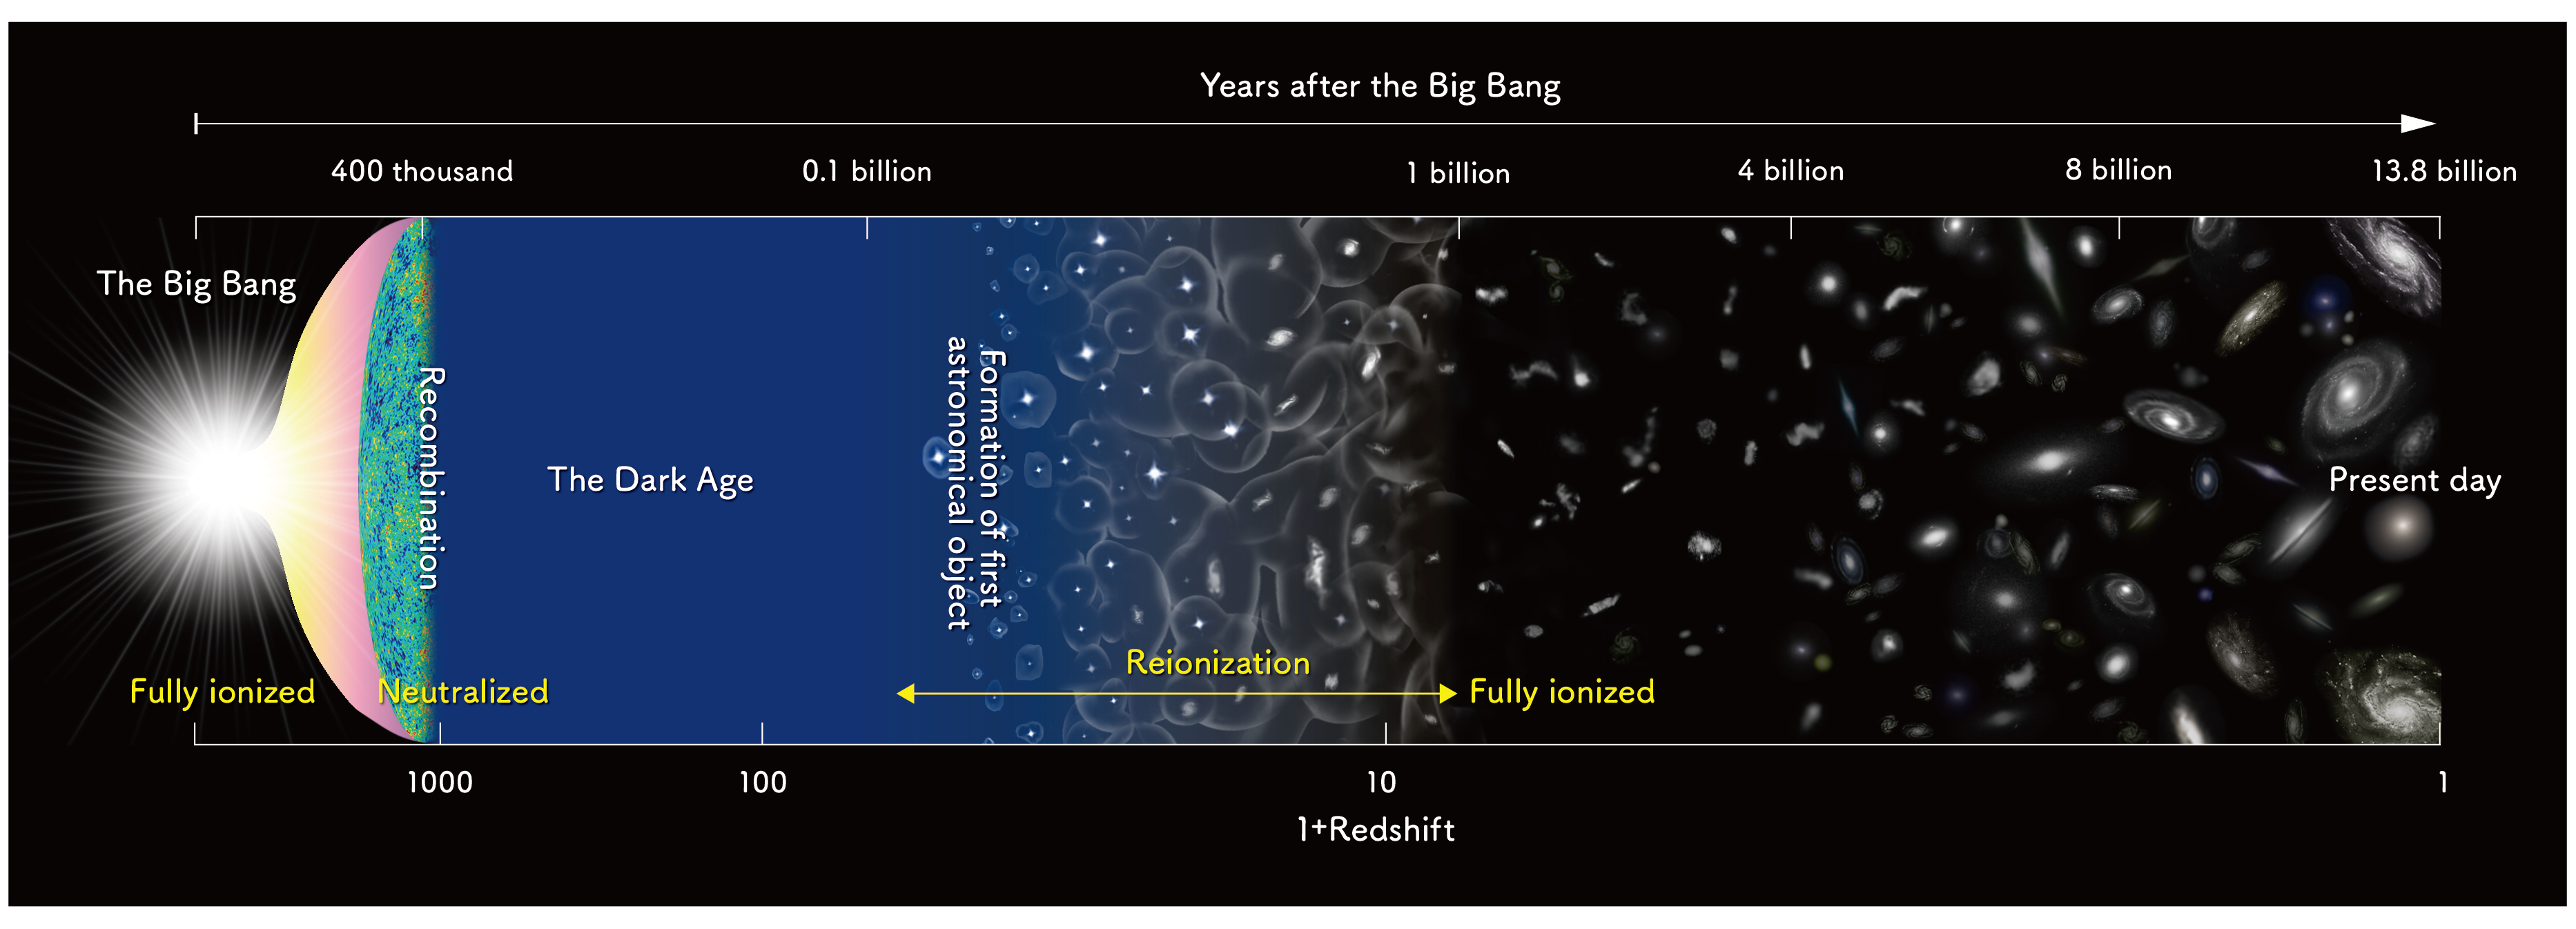
\includegraphics[width=0.95\linewidth]{Figures/Reionizationtimeline.jpg}\\
					\caption{Cosmic history of the Universe}
					\label{Fig:timeline}
				\end{center}
			\end{figure}
		
		Recombination (z $\approx1100$) occured when the HI was formed from the cool enough universe. Prior to that, electrons were not bound to protons, and the universe contained ionized plasma known as photon-baryon fluid. The CMB was then formed by decoupled photons. Subsequently, the neutral hydrogen (HI) became the dominant baryonic component of the intergalactic medium (IGM). This was prior to the formation of the first stars during the Dark Ages (z $\approx1100$ - z $\approx30$). There was rapid cooling of gas relative to the CMB. If the hydrogen dispersion can be mapped in this era, valuable cosmological data can be produced. \cite{2015Sci...349..849H, 11, 2004PhRvL..92u1301L}.\\
				
		 There were density fluctuations in the distribution
		 of matter (hydrogen), and the overdense regions collapsed under the	influence of gravity, ultimately creating the first stars. Thus, nuclear reaction resulted into Cosmic Dawn (z $\approx30$ - z $\approx10$). An ernomous emitted energy from the stars reionises the Universe causing ionisation, this further results in stars disintegrating due to gravitational disintegration leading to the formation of galaxies. There is a decelerating effect in the Universe expansion due to the force of gravity within dominating matter \cite{2015Sci...349..849H, 2017arXiv170808521D}.\\
				
		Through out the cosmological epochs, what is known is very minimal because it hasn't been straightforward to directly observe them. Nevertheless, the contemporary occurence of the \SI{21}{cm} cosmology has imparted the capability of bridging the gap  between what is known and what is not know about the eras of our history\cite{2014ApJ...782L...9V, 2013PhRvD..87d3002L}.
		
	\section{21 cm Spectral Line Generation and Experiments}
		Our Universe is rich in the hydrogen gas, hence a
		concerted effort in the experimental community to develop telescopes for mapping hydrogen via \SI{21}{cm} emission  wavelength line. The \SI{21}{cm} wavelength of hydrogen gas is being observed by several experiments which are modelled for the purpose of Hydrogen mapping in our Universe. This hydrogen line is a significant mechanism as it helps in the probing of the dark ages to the epoch of reionization (EoR) \cite{2013PhRvD..87d3002L,2014ApJ...782...66P}.The generation of the hydrogen line (\SI{21}{cm} line or HI line) is due to the intrinsic spin of the hydrogen atoms, namely, an electron and the proton \cite{book:832129} 
		
		The electron and proton spins can be oriented in either the opposing or the same direction respective to each other. When they are in an opposing direction they result in an antiparallel spin which implies that the hydrogen atom is in the lower energy state and when they are in the same direction, they result in a parallel spin, which implies that the hydrogen atom is in the higher energy state. Once an electron transition from one state to another, the hydrogen atom discharges a photon relative to \SI{21}{cm} wavelength equivalent to (\SI{1420}{MHz}). This process of transition is called the spin flip transition. Since our Universe is rich in hydrogen and has a potential of long wavelength radiation to penetrate dust, this \SI{21}{cm} radiation is an ideal tool for probing the history of the universe at any epoch of interest. \autoref{Fig:21cm}\footnote{https://www.skatelescope.org/radio-astronomy/} shows the spin flip transition process \cite{16, book:832129}.
		
			\begin{figure}[htb!]
				\begin{center}
					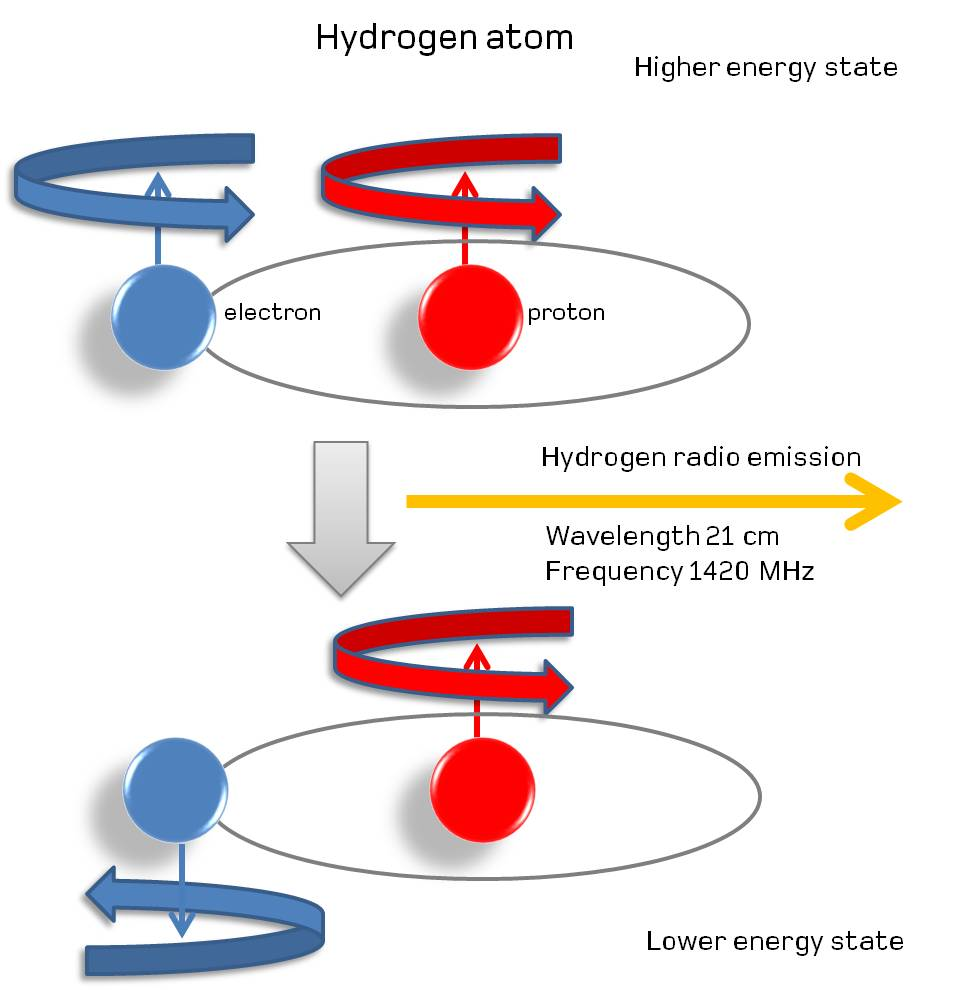
\includegraphics[width=0.5\linewidth]{Figures/Hydrogenemission1.jpeg}
					\caption{The formation of the 21 cm wavelength line by the process of spin flip transition where the hydrogen atom moves from one energy state to another}
					\label{Fig:21cm}
				\end{center}
			\end{figure}
			 
		The \SI{21}{cm} hydrogen line is redshifted extremely as it moves further away. It is redshifted as far as z $\approx1000$ which corresponds to the cosmological dark ages and is observable at low frequencies ranging from \SI{1.4}{MHz} to \SI{140}{MHz}. This is mathematically represented by the relationship between wavelength and redshift which is given by
		\begin{equation} \label{eq1.1}
		\begin{split}
		1+z & = \frac{\lambda_{obs}}{\lambda_{emit}}= \frac{1}{a}
		\end{split}
		\end{equation}
		where $z$ is the redshift, $\lambda_{obs}$ is the wavelength of the observed signal, $\lambda_{emit}$ is the wavelength of the emitted signal and $a$ is the Universe expansion scale factor. The ground based telescopes and experiments are faced with a challenge when it comes to using the \SI{21}{cm} highly redshifted line emission to observe the dark ages, cosmic dawn and the Epoch of Reionization \cite{2016ExA....41..271R}. This is due to the man made Radio Frequency Interference (RFI), ionospheric interferences, the Galactic emission, the instrumental systematics and the ionosphere which is non transparent below \SI{10}{MHz}. In order to minimize RFI and ionospheric contamination, there have been proposals to observe long wavelengths from space based telescopes further away from the ionosphere of our planet. These space based telescopes don't exist yet, and there are a number of ground-based experimental efforts to understand how well we can make measurements from Earth \cite{2016ExA....41..271R}.\\ 
		
		A number of experiments use the \SI{21}{cm} Hydrogen line to study the evolution of the Universe. These experiments are aimed at observing different epochs of the Universe including Dark Ages (z $\approx1100$ - z $\approx30$), cosmic dawn z $\approx30$ - z $\approx10$) and Epoch of Reionization z $\approx10$ - z $\approx2.5$). The Long Wavelength Array (LWA) experiment operating at a frequency range of \SI{10}{MHz} to \SI{88}{MHz} is in correspondence with the redshift of $15<\text{z}<142$ and is aimed at probing the cosmic dawn and the dark ages \cite{2010iska.meetE..24H}, the other experiments with the same aim are the EDGES \cite{2018AAS...23111604M}, the PRIZM \cite{2018arXiv180609531P} experiment probes the cosmic dawn only. The frequency and redshift ranges are shown in \autoref{table:range}. OVRO-LWA \cite{2018AJ....156...32E} probes EoR to cosmic dawn. GMRT-EoR \cite{2013MNRAS.433..639P}, PAPER \cite{2010AJ....139.1468P},MWA \cite{2009IEEEP..97.1497L} and HERA \cite{2017PASP..129d5001D} probes EoR. LOFAR \cite{2013A&A...556A...2V} probes from the Era of Acceleration to the Dark Ages. The frequency and redshift ranges are shown in \autoref{table:range1}. \\			
	

\begin{table}[h!]
	\centering
	\begin{tabular}{|c | c | c | c| c|} 
		\hline
		 & EDGES &  PRIZM & LWA \\ [0.5ex] 
		\hline
		Frequency Range (MHz) & 50 - 190 & 70 - 100 & 10 - 88\\
		\hline
		Redshift Range & $\approx$ 28 - 6.5 & $\approx$ 19 - 13 & $\approx$ 142 - 15 \\
		\hline
		\end{tabular}
	\caption{EDGES, PRIZM and LWA frequency and redshift ranges}
	\label{table:range}
\end{table}
	
\begin{table}[h!]
	\centering
	\begin{tabular}{|c | c | c | c | c | c |} 
		\hline
		& GMRT-EoR &  PAPER & MWA & HERA & LOFAR\\ [0.5ex] 
		\hline
		Frequency Range (MHz) & 150 & 139 - 174 & 70 - 300 & 50 - 250 & 10 - 240\\
		\hline
		Redshift Range & $\approx$ 8.5 & $\approx$ 9 - 7 & $\approx$ 19 - 4 & $\approx$ 6 - 30 & $\approx$ 142 - 5 \\
		\hline
	\end{tabular}
	\caption{GMRT-EoR, PAPER, MWA, HERA and LOFAR frequency and redshift ranges}
	\label{table:range1}
\end{table}
	
	
\section{Long Wavelength Astronomy}
\subsection{Background/History of Long Wavelength Astronomy}
	The father of radio astronomy, Karl G. Jansky played a vast role in the inauguration of radio astronomy which is dated back to 1931. At that time he was an employee at the Bell Telephone Laboratories as a radio engineer. Jansky was allocated to study and solve the problem that hindered the radio communication systems. Using highly directive antenna arrays shown in \autoref{Fig:Jansky}, he discovered that the radio frequency noise that hindered the communication systems was caused by the static from the thunderstorms \cite{book:BasicsofRA,book:RA}. \\
	
	\begin{figure}[htb]
		\begin{center}
			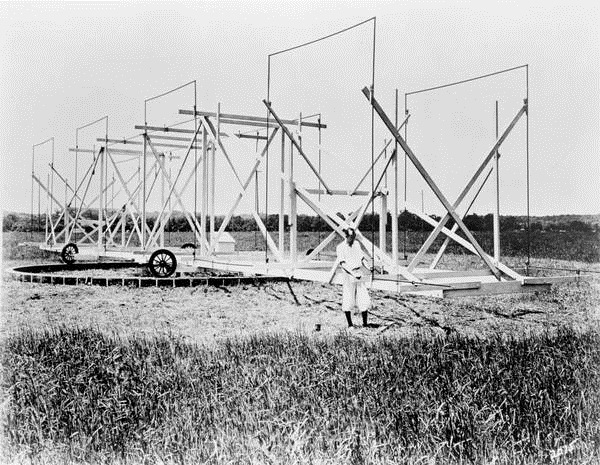
\includegraphics[width=0.7\linewidth]{Figures/jansky1.jpg}
			\caption{Jansky's highly directive antenna arrays which he used to discover the cause of RFI that hindered the communication systems at Bell Telephone Laboratories  \cite{book:BasicsofRA}}.
			\label{Fig:Jansky}
		\end{center}
	\end{figure}
	The contraption that he constructed operated at an approximated frequency of \SI{20}{MHz} corresponding to an approximate long wavelength of \SI{15}{m}. He further found radio radiation from the Galactic Center at the operating frequency. Out of interest in Jansky's instigating discoveries, Grote Reber designed a radio telescope that operated at a range of approximately \SI{10}{MHz} to \SI{160}{MHz} (\SI{30}{m}-\SI{2}{m} wavelength) in 1937. He discovered that the powerful source at longer wavelengths was the Milky Way area . Furthermore, he realised that the radio telescope \textit{"acts like a bolometer, or heat-measuring device, in which the radiation resistance of the antenna measures an equivalent temperature of distant part of space to which it is projected by the 24 antenna response pattern"} \cite{1988JRASC..82...93R,CosmicStatic,2012PASP..124.1090H}.\\[0.1cm]
	
	Because of the research which was done for the communication systems, astronomy was born and has expanded to fields of radio astronomy and astrophysics. \cite{2012PASP..124.1090H}. This led to an accelerated discovery of the hydrogen line research area which was allocated an operating frequency of \SI{1420}{MHz} (\SI{21}{cm} wavelength). The greatest significance which has been formed by research at the hydrogen line is enormous to radio astronomy and its observables \cite{10.2307/530765}. After all these discoveries, the long wavelength astronomy fascination has been resuscitated in the present epoch.
	\subsection{Modern/Current Long Wavelength Astronomy/Experiments}
		Over the last ten years, there has been funds allocated to the long wavelength experiments which exists and which are yet to be. There is quite a few low frequency experiments, but this document will briefly discuss LWA (\autoref{Fig:LWA}\footnote{https://phys.org/news/2011-01-astronomer-field.html}) based in the Very Large Array (VLA site). Further discussion will be on the few measurements that exists at $\lessapprox$ 30 MHz. Two of these experiments represent the lowest frequencies measured to date (Reber's antenna, RAE-B), and the other two represent the highest resolutions achieved in this frequency range (DRAO, OVRO-LWA).\\
		
		{\bf LWA:} It is based in New Mexico on the Very Large Array (VLA) site. Its operating frequency ranges between \SI{10}{MHz} - \SI{88}{MHz} (wavelength between \SI{30}{m}- \SI{3.41}{m}) and is made up of incoporated beams which are from digitized 258 dual polarisation dipoles. The functionality of the first station of this project was finalised in 2011. The LWA possess distinctive multiskilled abilities of measuring cosmic evolution, astrophysical plasma, relativistic particles, decametric radio radiation from Jupiter - like extrasolar planets and giant flares from magnetars. The final LWA is aimed at consisting of 53 phased array stations which are steered electronically with as far as \SI{400}{km} baseline \cite{2012JAI.....150004T,2010iska.meetE..24H}. This experiment observes the Northern and Western sky and the ALBATROS - EGG probes the Southern sky.\\
		
		
		\begin{figure}[h!]
			\begin{center}
				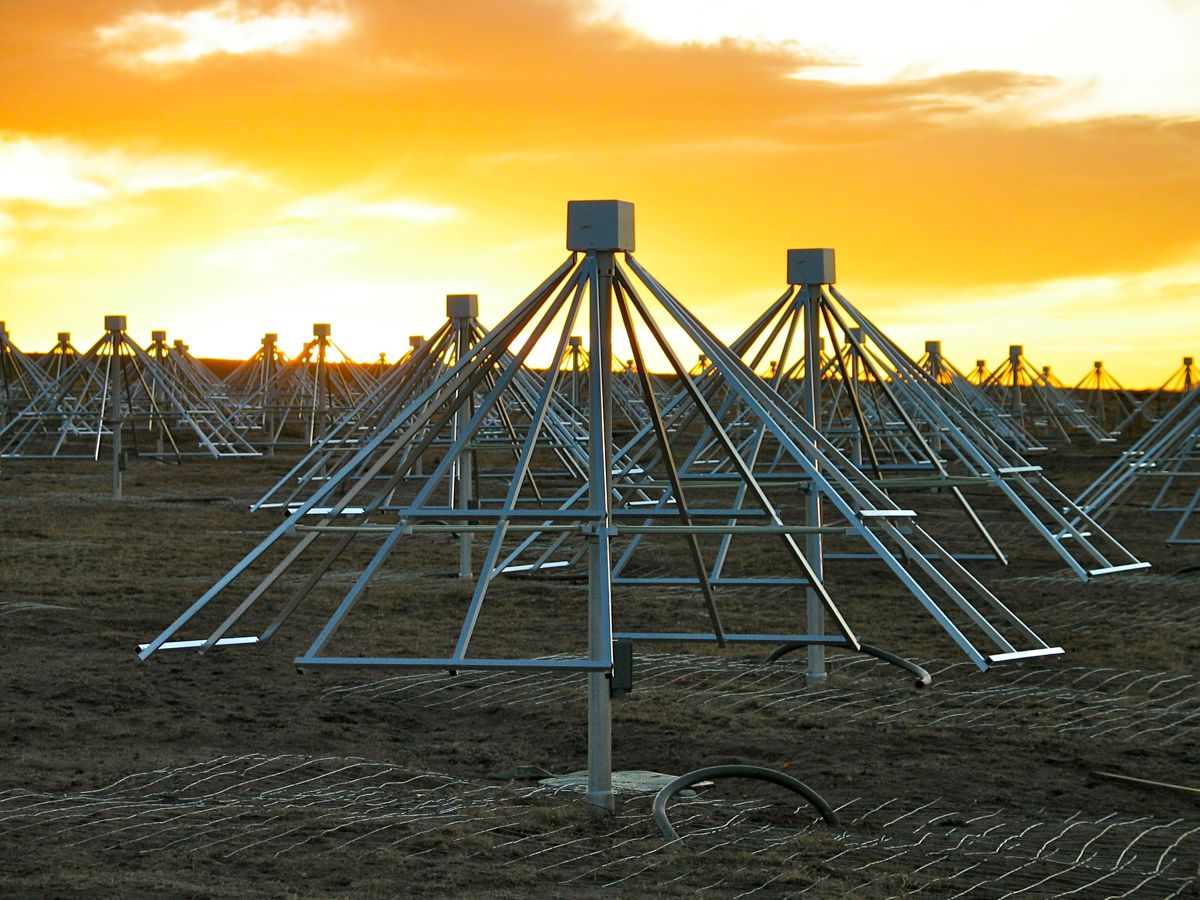
\includegraphics[width=0.5\linewidth]{Figures/LWA.jpg}
				\caption{Several LWA Telescopes in New Mexico (VLA site)}
				\label{Fig:LWA}
			\end{center}
		\end{figure}
		
		\begin{figure}[htb]
			\begin{center}
				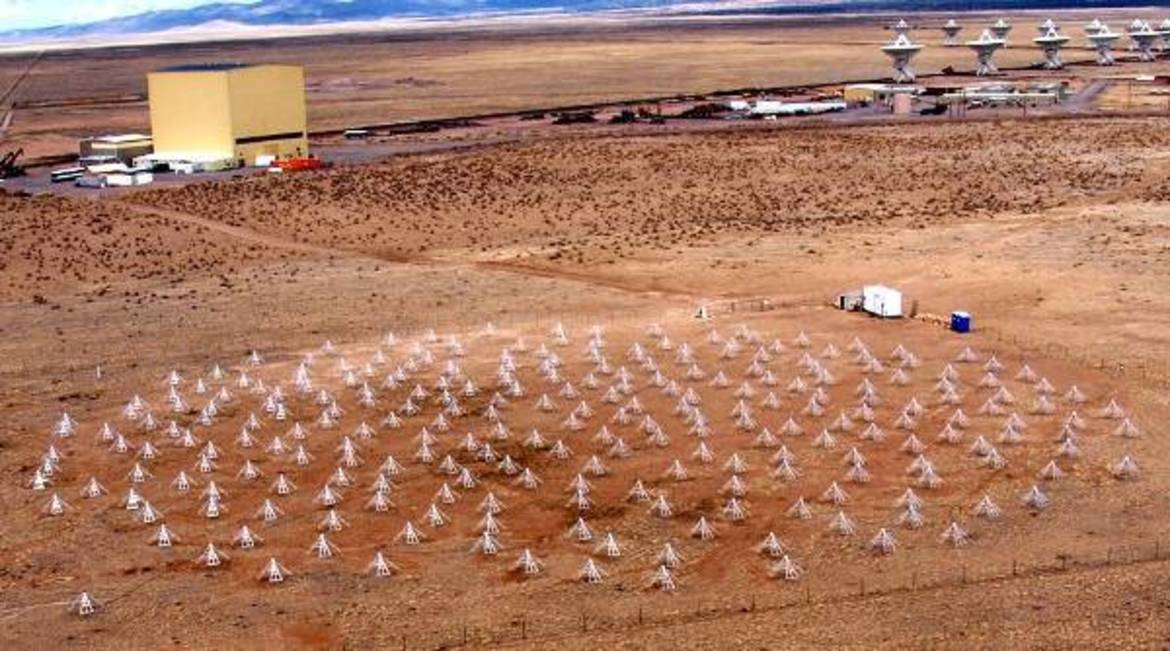
\includegraphics[width=0.7\linewidth]{Figures/LWA256.jpg}
				\caption{All 256 LWA Telescopes in New Mexico (VLA site) \cite{2012PASP..124.1090H}}
				\label{Fig:LWA256}
			\end{center}
		\end{figure}
		
Comprehensive reviews of experimental efforts exist elsewhere but none of them has made measurements at the lowest frequencies of $\lessapprox$ 30 MHz. This is due to the challenges namely, the ionosphere, RFI, Galactic emission and instrumental systematics \cite{2018arXiv180609531P}. \\

Grote Reber came up with the state of art by constructing a telescope which operated at very low frequencies between 0.52 MHz and 2.1 MHz, which had 192 dipoles. At 2.1 MHz it had a resolution of as low as $\approx$5 deg. The key map of the sky was created by this experiment at 2.1 MHz. He also mentioned that his measurements were influenced by galactic emission and the ionosphere \cite{article, 1988A&A...195..372W}. The Radio Astronomoy Explorer-2 (RAE-2) have very low operating frequency ranges between of 25 kHz - 13 MHz, it main science goal was to do radio astronomy evaluation of our Galaxy (the Milkyway), the Sun and all the planets including Earth. The resolution of this experiment is $\approx$10 deg at 4.7 MHz \cite{1975A&A....40..365A}. Both of these experiments made very low resolution measurements.\\

The experiments which made the high resolution measurements are the  Dominion Radio Astrophysical Observatory (DRAO) 22 MHz telescope and the OVRO-LWA 36 MHz experiment. The DRAO operates at 22 MHz and its resolution ranges between $\approx$1.1 deg - 1.7 deg. Its main science goal was to measure the emission from discrete sources and to observe our Galaxy's emission from its environment \cite{1999A&AS..137....7R}. The OVRO-LWA operates at frequency ranges of 36.528 MHz and 73.152 MHz. At these frequencies it has an angular resolution of \SI{15}{\arcminute} \cite{2018AJ....156...32E}. ALBATROS aims at attempting to do high resolution measurements at a frequency of $<$20 MHz since there's none as yet.
		
\chapter{ALBATROS - EGG Instrumentation}
\section{ALBATROS - EGG Overview}
		
The Array of Long Baseline Antennas for Taking Radio Observations from the Sub-antarctic- Exploratory Gizmo on the Ground (ALBATROS-EGG) is a recently deployed two element inteferometer which is making exploratory measurements at a frequency range of \SI{1.2}{MHz}- \SI{81}{MHz} separated by a baseline of \SI{110}{m}. It was deployed in Marion Island in April 2018 as shown in \autoref{Fig:ALBATROS-EGG}. This experiment (ALBATROS-EGG) uses the LWA hardware.  The existing systems had to be optimised for better operational effeciency and effectiveness. Since this is an ongoing project, many other optimisation techniques are yet to be employed for the deployment in April 2019. \\

The final project (ALBATROS) is aimed at consisting of autonomous antenna stations that will map the low frequency sky. Since these experiments are exploratory, they are taking steps towards achieving the future objective of probing the Dark Ages.The ALBATROS stations (huts) will be separated by baselines of \SI{\approx {20}}{km} as shown in \autoref{Fig:Marion}. Marion Island huts which are potential stations for the ALBATROS have a ring-like pattern which is appropriate for imaging and produces a FWHM synthesized beam of 8' at 5 MHz as shown in \autoref{Fig:10}. This beam is a natoable advancement over existing measurements to date.The ALBATROS main goal thus far will be to attempt to map high resolutions at low frequencies which crucial before moving in to the cosmology of measuring the dark ages. The two-element interferomentric pathfinder is not yet operating autonomously, it uses the direct cross correlation technique whereas the yet to be ALBATROS will write the lowest 10 - 20 MHz baseband to disk then gets correlated afterwards.\\

		\begin{figure}[!ht]
			\begin{center}
				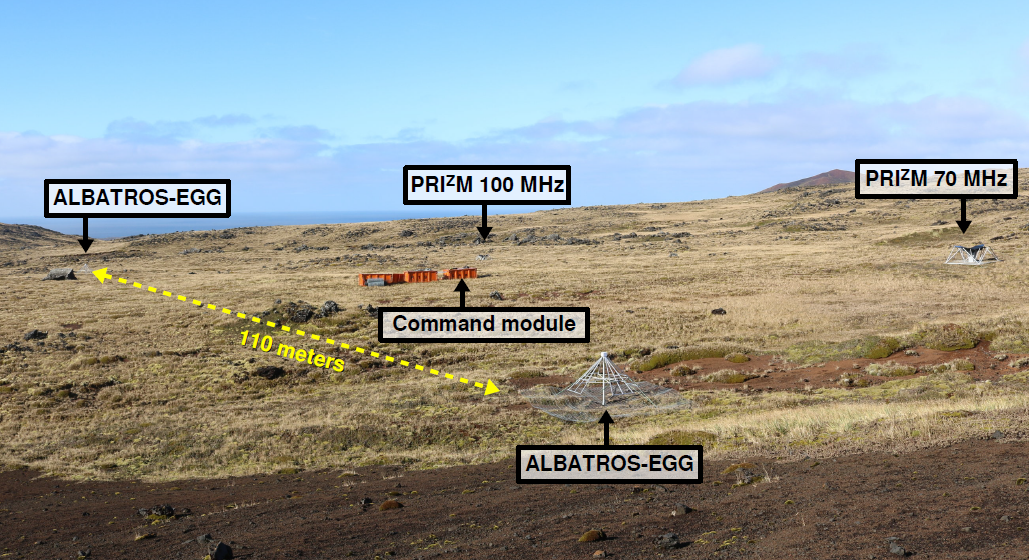
\includegraphics[width=1\linewidth]{Figures/ALBATROS-EGG.PNG}
				\caption{The ALBATROS-EGG pathfinder installed at the PRIZM site on Marion Island. The pathfinder comprises two 	dual-polarization antennas separated by roughly 110 m on an	east-west baseline. Long coaxial cables connect the antennas to	an orange shipping container that houses the readout electronics and serves as our "command module".}
				\label{Fig:ALBATROS-EGG}
			\end{center}
		\end{figure}
			
		\begin{figure}[!htb]
			\centering
			\begin{subfigure}{.58\textwidth}
				\centering
				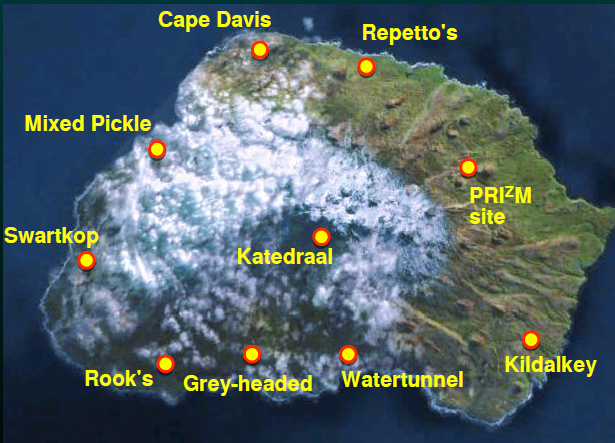
\includegraphics[width=.9\linewidth]{Figures/site.PNG}
				\caption{Marion Island huts which are potential stations for the ALBATROS. The ring-like pattern is appropriate for imaging and produces a FWHM synthesized beam of 8' at 5 MHz.}
				\label{Fig:Marion}
			\end{subfigure}%
			\begin{subfigure}{.45\textwidth}
				\centering
				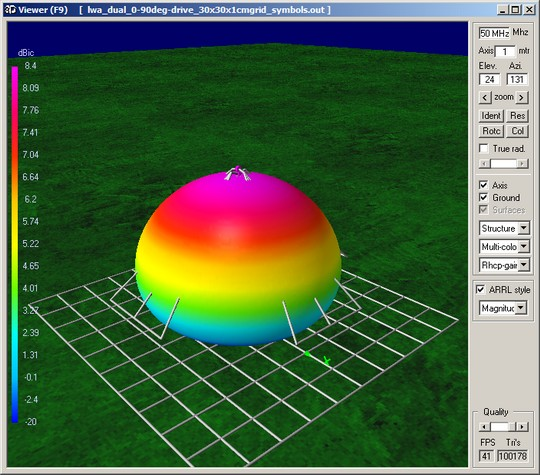
\includegraphics[width=.9\linewidth]{Figures/beam.png}
				\caption{Omnidirectional, dome shaped beam pattern which promises an improved resolution over the existing experiments to date.}
				\label{Fig:beam}
			\end{subfigure}
			\caption{Potential stations and a beam encouraging enough to implement ALBATROS experiment}
			\label{Fig:10}
		\end{figure}
		
The ALBATROS-EGG schematic is shown in \autoref{Fig:ALBATROS-EGG Schematic}. The system uses the dually polarised dipole like antennas which are omidirectionally patterned. The front end electonics (FEE) are configured in a printed circuit board (PCB) which makes it easy for them to be mounted on the supporting structure of the antennas. The gain of the FEE is $\approx$35 dB and its noise figure (NF) ranges between $\approx$2.7 dB and 2.9 dB. From the FEE PCB, a coaxial cable sends the signal thnrough to the bias tee which extracts both the RF and the DC without any degradation. \newline The high pass and the low pass filter rejects the low frequency signals and high frequency signals respectively. The signal is then amplified by a $\approx$20 dB amplifier which then send the amplified signals to the Smart Network ADC Processor (SNAP) board which does the readouts and does a series of processing step. The raspberry pi interacts with the SNAP board for data storage.  This schematic is an illustration of what already exists in Marion Island for the two-element interferometric array. However, for the autonomous stations, the layout is going to be revised. 

 		
		\begin{figure}[!ht]
				\begin{center}
					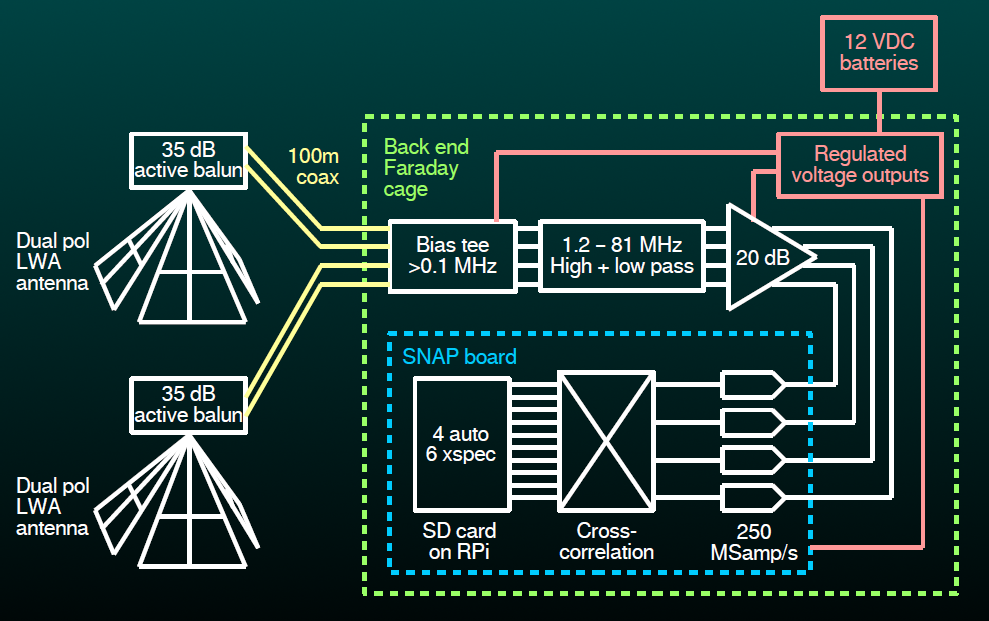
\includegraphics[width=0.9\linewidth]{Figures/ALBATROS-EGG-Schematic.PNG}
					\caption{ALBATROS - EGG pathfinder schematic which consists of the dual polarisation antennas, the 35 dB gain FEE, the 100 m coaxial cable which connects the FEE to the back end Faraday cage which comprises of the bias tee, HPF, LPF, amplifier, snap board and regulated voltage outputs which are powered by 12 VDC batteries.}
					\label{Fig:ALBATROS-EGG Schematic}
				\end{center}
		\end{figure}
			
			
	\newpage
	\newpage	
	\section{System Signal Chain}	
	The single antenna analog signal chain is shown in \autoref{Fig:Signal Chain}. The components of the system are discussed in detail as per the block diagram illustrated in \autoref{Fig:Signal Chain}. This analog signal chain is a proposed outline of how the autonomous stations will be configured. There might be changes to the block diagram at a later stage should there be a need to revise it for the stations.
		
		\begin{figure}[htb]
			\begin{center}
				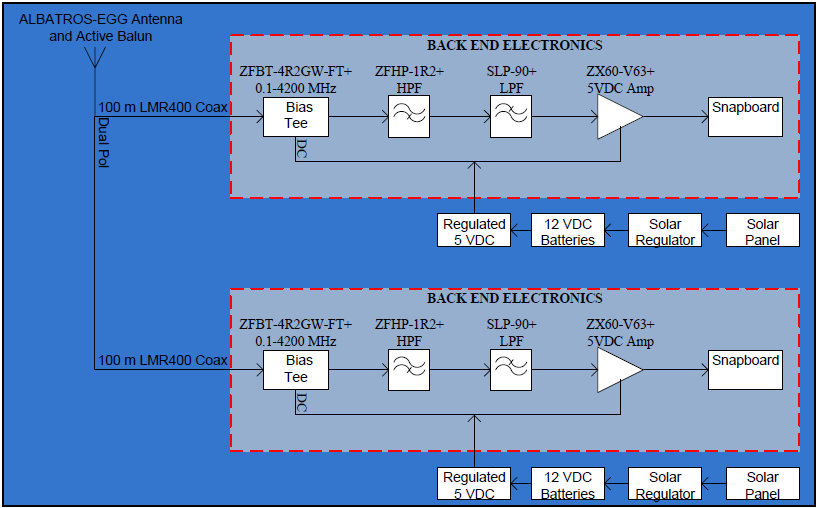
\includegraphics[width=1.0\linewidth]{Figures/Signal-Chain.png}
				\caption{Proposed analog signal chain block diagram for the yet to be experiment, the ALBATROS}
				\label{Fig:Signal Chain}
			\end{center}
		\end{figure}
	
	\subsection{Antenna}	
	The dipole like antennas are of high preference for this project because they are relatively simple and they are omnidirectionally patterned \cite{Memo28}. Becuase of these kind of antennas possessing low gain, the Galactic noise is limited by a fraction of 10 and the unwanted harmonics and intermodulation products are prevented \cite{Memo28,Memo27}.\\
	
	\subsection{Front End Electronics (FEE)}
	All the front end components were incorporated for in a double sided printed circuit board (PCB) as shown in \autoref{Fig:Balun} and the block diagram is shown in \autoref{Fig:Balun Schematic}. The Monolithic Microwave Integrated Circuits (MMICs) is the used design for the PCB. One side of the PCB is populated with components and the other side is a solid copper ground plane aperiodically stitched to the grounded copper on the side populated with components. The receiver system is made up of the active balun, filter and the gain stage that connects to the \SI{100}{m} coaxial cable which is connected to the back end \cite{2012PASP..124.1090H}.\\ 
	The input impedance (Z\textsubscript{o}) of \SI{50}{\ohm} is introduced to the dipole by the active balun. The signal is then fed through an amplifier which amplifies it by +24 dB of gain. The balanced signal is then converted to unbalanced through a 180 \degree hybrid coupler. The band pass filter (BPF) receives the single ended signal in order for it to reject all the frequencies which are not within the range of interest. The signal gets fed to a second amplifier which again amplies it by +24 dB of gain and the output impedance of the FEE is matched to a \SI{50}{\ohm} coaxial cable. The bias tee is responsible for providing power to the FEE and extracts the RF signal by the use of the coaxial cable. This unit has an overall gain of $\approx$ 35 dB and an overall noise figure of $\approx$ 2.7 dB to $\approx$ 2.9 dB \cite{Memo35}.
	
	\begin{figure}[htb]
		\begin{center}
			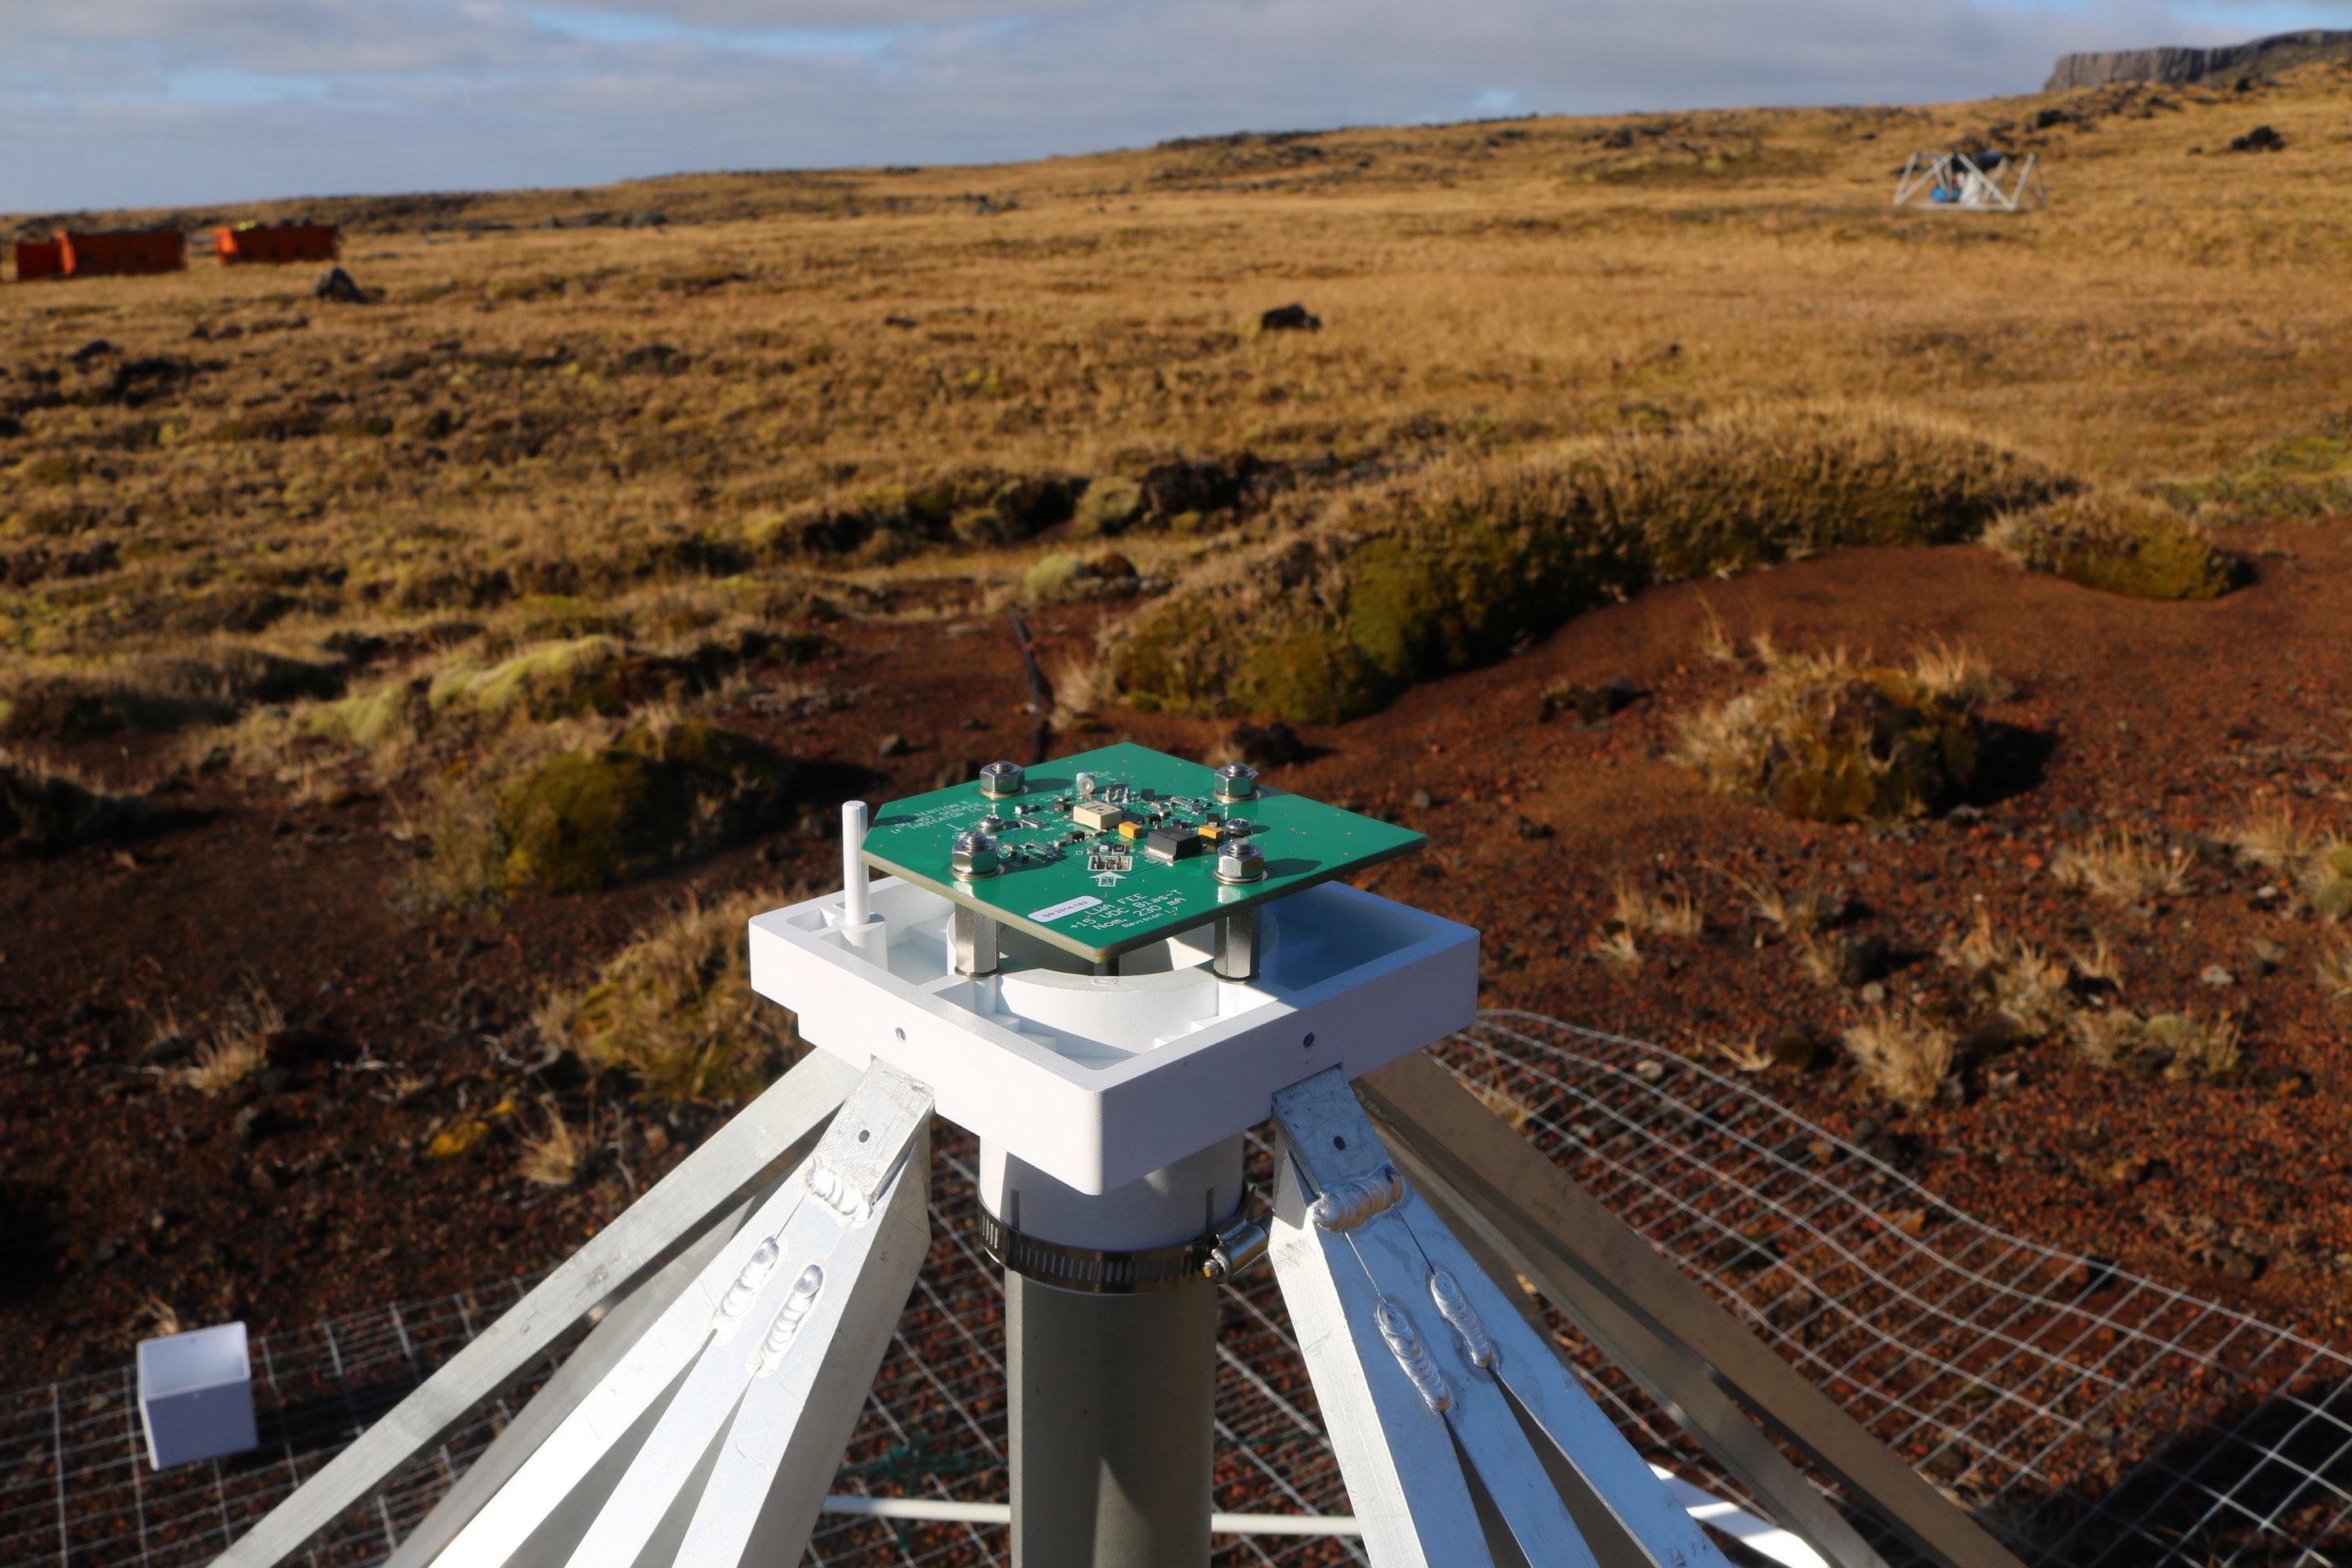
\includegraphics[width=1.0\linewidth]{Figures/balun.jpg}
			\caption{Unenclosed FEE mounted on the ALBATROS-EGG antenna supporting structure.} 
			\label{Fig:Balun}
		\end{center}
	\end{figure}
	
	\begin{figure}[h!]
		\begin{center}
			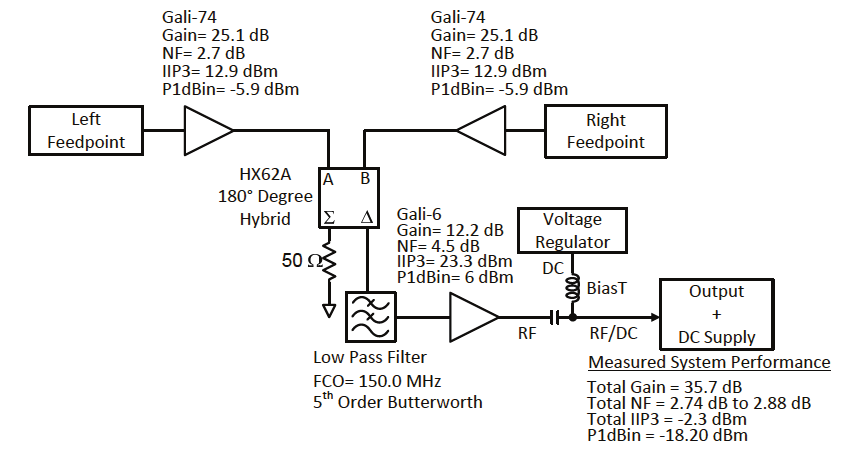
\includegraphics[width=0.7\linewidth]{Figures/Balun_Block.png}
			\caption{One Polarisation Block Diagram of the FEE \cite{2012PASP..124.1090H}}
			\label{Fig:Balun Schematic}
		\end{center}
	\end{figure}
	
	\newpage
	\subsection{Back End Electronics}	
	The back end electronics consists of the bias tee, high pass filter (HPF), low pass filter (LPF) and the Smart Network ADC Processor (SNAP) board. \\

	\textbf{Bias Tee} - The bias tee is a network made up of 3 ports \footnote{https://www.pasternack.com/bias-tees-category.aspx}. It is used to extract the RF signal from a \SI{100}{m} LMR400 coaxial cable which has a nominal attenuation of \SI{\approx 0.4}{dB/\SI{100}{m}} - \SI{\approx 3.7}{dB/\SI{100}{m}} at \SI{1.2}{MHz} - \SI{81}{MHz} respectively \footnote{https://www.timesmicrowave.com/documents/resources/LMR-400.pdf}. The bias tee which is used is the Mini Circuits device ZFBT-4R2GW-FT+ which operates between \SI{0.14}{MHz} - \SI{4200}{MHz}. It has an insertion loss of 0.16 dB at centre frequency of  \SI{\approx 10}{MHz} as per the datasheet \footnote{https://www.minicircuits.com/pdfs/ZFBT-4R2GW-FT+.pdf}.\\
	
	\textbf{HPF} - The HPF rejects any signals with low frequencies and allow through signals with high frequencies \footnote{http://www.learningaboutelectronics.com/Articles/High-pass-filter.php}. The HPF used is the ZFHP-1R2+ Mini Circuits device which operates between  \SI{1.2}{MHz} - \SI{800}{MHz}. It has a nominal insertion loss of $\approx$ 0.2 dB at centre frequency of  \SI{\approx10}{MHz} as per the datasheet \footnote{https://www.minicircuits.com/pdfs/ZFHP-1R2+.pdf}.\\
	
	\textbf{LPF} - The LPF rejects all signals with high frequencies and allows all signals with low frequencies \footnote{http://www.learningaboutelectronics.com/Articles/Low-pass-filter.php}. The LPF used is the SLP-90+ Mini Circuits device which operates between \SI{1}{MHz} - \SI{400}{MHz}. It has a nominal insertion loss of $\approx$ 0.14 dB at the centre frequency of  \SI{\approx 10}{MHz} \footnote{https://www.minicircuits.com/pdfs/SLP-90+.pdf}.\\
	
	\textbf{Amplifier} - The amplifier at the backend amplifies the signal which is sent through to the snapboard by the gain of +20 dB. The amplifier used is the Mini CIrcuits device ZX60-V63+ which operates at a frequency range of \SI{0.05}{GHz} - \SI{6}{GHz}. It has a noise figure of $\approx$ 3.6 dB at its lowest operating frequency of \SI{\approx 50}{MHz} \footnote{https://www.minicircuits.com/pdfs/ZX60-V63+.pdf}.\\
	
	\textbf{SNAP Board} - The SNAP board used is specified by \footnote{http://www.xilinx.com/products/silicon-devices/fpga/kintex-7.html}. The  SNAP board samples the signals it receives by 250 Msampl/s using internal ADCs where the signal of the clock is from the Valon 5007 frerquency synthesizer module. This creates a frequency range between 0 - 125 MHz which contains 2048 channels. A SNAP board interacts with a raspberry pi and that is where the data is saved.\\

	\subsection{Solar Power Supply System}
	
	A solar power system was proposed over the current power system which uses a generator to charge the batteries. The current power system of the ALBATROS-EGG uses generators to charge the batteries (2x 12VDC 200 Ah) manually every once in a number of days. From the observation that has been made, the batteries take $\approx$ 2 days to discharge to a point where the system shuts down. Because of the weather conditions in Marion Island, an individual can sometimes be unable to go to site, which means that if the weather does not allow, the system can be shut down for a longer period. Thus, a solar power system solution was proposed so that the system can continously run without having to be recharged manually.\\
	
	As part of the solar power system development, a power budget had to be made, the RFI generated by the power system had to be considered together with the mechanical footprints. The power budget is shown in \autoref{table:budget}. 
	
	\begin{table}[h!]
		\centering
		\begin{tabular}{|c | c | c | c |} 
			\hline
			Module & Power Dissipation (Watts) &  Voltage (Volts) & Current (Amperes)\\ [0.5ex] 
			\hline
			SNAP board & $\approx$30 & 12 & 2.5\\
			\hline
			FEE and Dual Pol & $\approx$8 & 16 & 0.48 \\
			\hline
			2nd Stage Amplifier & $\approx$0.7 & 5 & 0.14\\
			\hline
			5007 Frequency Synthesizer & $\approx$2 & 5 & 0.4\\
			\hline
			RPi & $\approx$12.5 & 5 & 2.5 \\
			\hline
			\textbf{Total} & $\approx$53.2 &  & $\approx$6 \\
			\hline
		\end{tabular}
		\caption{The two-element pathfinder system ratings}
		\label{table:budget}
	\end{table}
	
	In the electronic systems, one always needs to make compensation because in real life the theoritical values may not be as practical as you have expected due to different factors that contribute to the electronic systems. Thus, a 15 W was added to the total power of the system in case we want to add one of the modules (an RPi for example) while the system is up and running . This added up to a rounded off total of $\approx$70 W.\\
		
	The proposed solar power supply system consists of the solar panel, solar charge controller, 12 VDC 150 Ah batteries\footnote{http://www.sacredsun.com/Upload/products/pdf/SP/12SP150.pdf} and regulated VDC. The proposed power system will be used to power the whole signal chain of the receiver. It is going to be used because it does not require an individual to consistently go to the site to power on the generator for battery charging.\\
	
	The prototype of the proposed system was tested on the roof of H Block at the University of KwaZulu Natal (UKZN). The solar panel which was used was the Enersol 300 which is capable of producing a maximum power voltage of 37.3 V and 8.2 A when operating at maximum power \footnote{https://cdn.shopify.com/s/files/1/1776/7837/files/Enersol300.pdf?9001617694037873925}. The solar charge controller which was used was the Victon Energy BlueSolar Maximum Power Point Tracking (MPPT) Charge Controller 75 V/15 A. This solar regulator can be used for 12 V and 24 V systems. It can also indicate the state of charge of the battery using the LEDs \footnote{https://www.victronenergy.com/upload/documents/Manual-BlueSolar-charge-controller-MPPT-75-10-75-15--100-15-EN-NL-FR-DE-ES-SE-ul.pdf}. In addition, this solar regulator and systems connected to it can be monitored by means of serial communication. Further details about the solar power supply system will be given	in the following chapter.
	
	
	
\newpage		
\chapter{Measurements and Results}

\section{Solar Power Supply System}
\subsection{Discussion}

Calculations had to be done to verify if the solar panel power supply system would be able to supply enough power to the system. The batteries provide +12 VDC to the ALBATROS-EGG system. This voltage is distributed to all units of the system, namely, the FEE, amplifier, the valon\footnote{http://docplayer.net/52408728-5007-dual-mhz-frequency-synthesizer-module-valon-technology-llc.html} which is configured together with the snap board and the raspberry pi(Rpi)\footnote{https://cdn.sparkfun.com/datasheets/Dev/RaspberryPi/2020826.pdf}. With reference to the existing system, the total current which the system draws when it is operational is $\approx$6 A. However, it should be noted that the approximated 6 A is for the existing pathfinder and it is used as a reference to design the autonomous stations power supply system, of which it is not yet known how much current will it draw.\\

Considering that the weather in Marion Island is mostly cloudy, the worst case scenario would be to have no sunlight at all for the whole day (24 hrs). Thus, the ampere hour rating required in a day to power the system is at least 144 Ah. Since a single battery has 150 Ah rating, it can be able to insufficiently power the system. The solar panel power system prototype was setup as shown in \autoref{Fig:Rooftop} in order to verify the calculations made and the functionality. This system dissipates a power of $\approx$70 W. The test set up was left on the roof for approximately a week while storing data in the Rpi as text files. The test set up consisted of 

\begin{enumerate}
	\item The solar panel which is the main supplier to the system,
	\item The solar regulator which was monitored via a communication port in order to be up to date with the whole system performance,
	\item A single +12 VDC 150 Ah battery which was going to be charged to provide power to the load. The other battery which was in the lab couldn't be used because the weather proof enclosure was only able to fit in one battery,
	\item The Arduino board which was programmed for serial to Universal Serial Bus (USB) communication,
	\item The Rpi which was connected to the sdr clock module for proper timing and syncronisation stored the data which was monitored from the solar regulator,
	\item The DC-DC converter is the stage of voltage regulation to the \SI{6}{\ohm} high power resistor. Both of these at as a load since the both dissipate power.
\end{enumerate}

\autoref{Fig:Rooftop1} and \autoref{Fig:Rooftop2} show the solar panel wires going to the weatherproof enclosure and the interior of the enclosure respectively.
 
\begin{figure}[h!]
	\begin{center}
		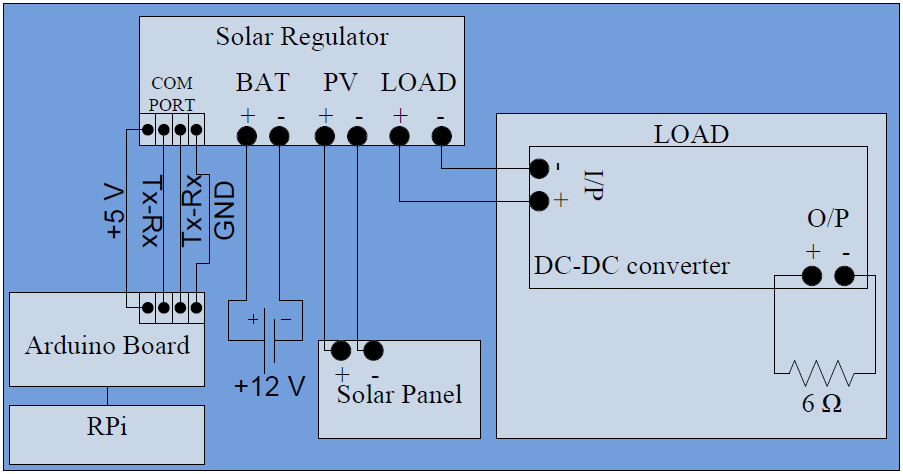
\includegraphics[width=0.8\linewidth]{Figures/Rooftop.PNG}
		\caption{Solar Power System Rooftop Test Set Up Block Diagram}
		\label{Fig:Rooftop}
	\end{center}
\end{figure}

\begin{figure}[h!]
	\begin{center}
		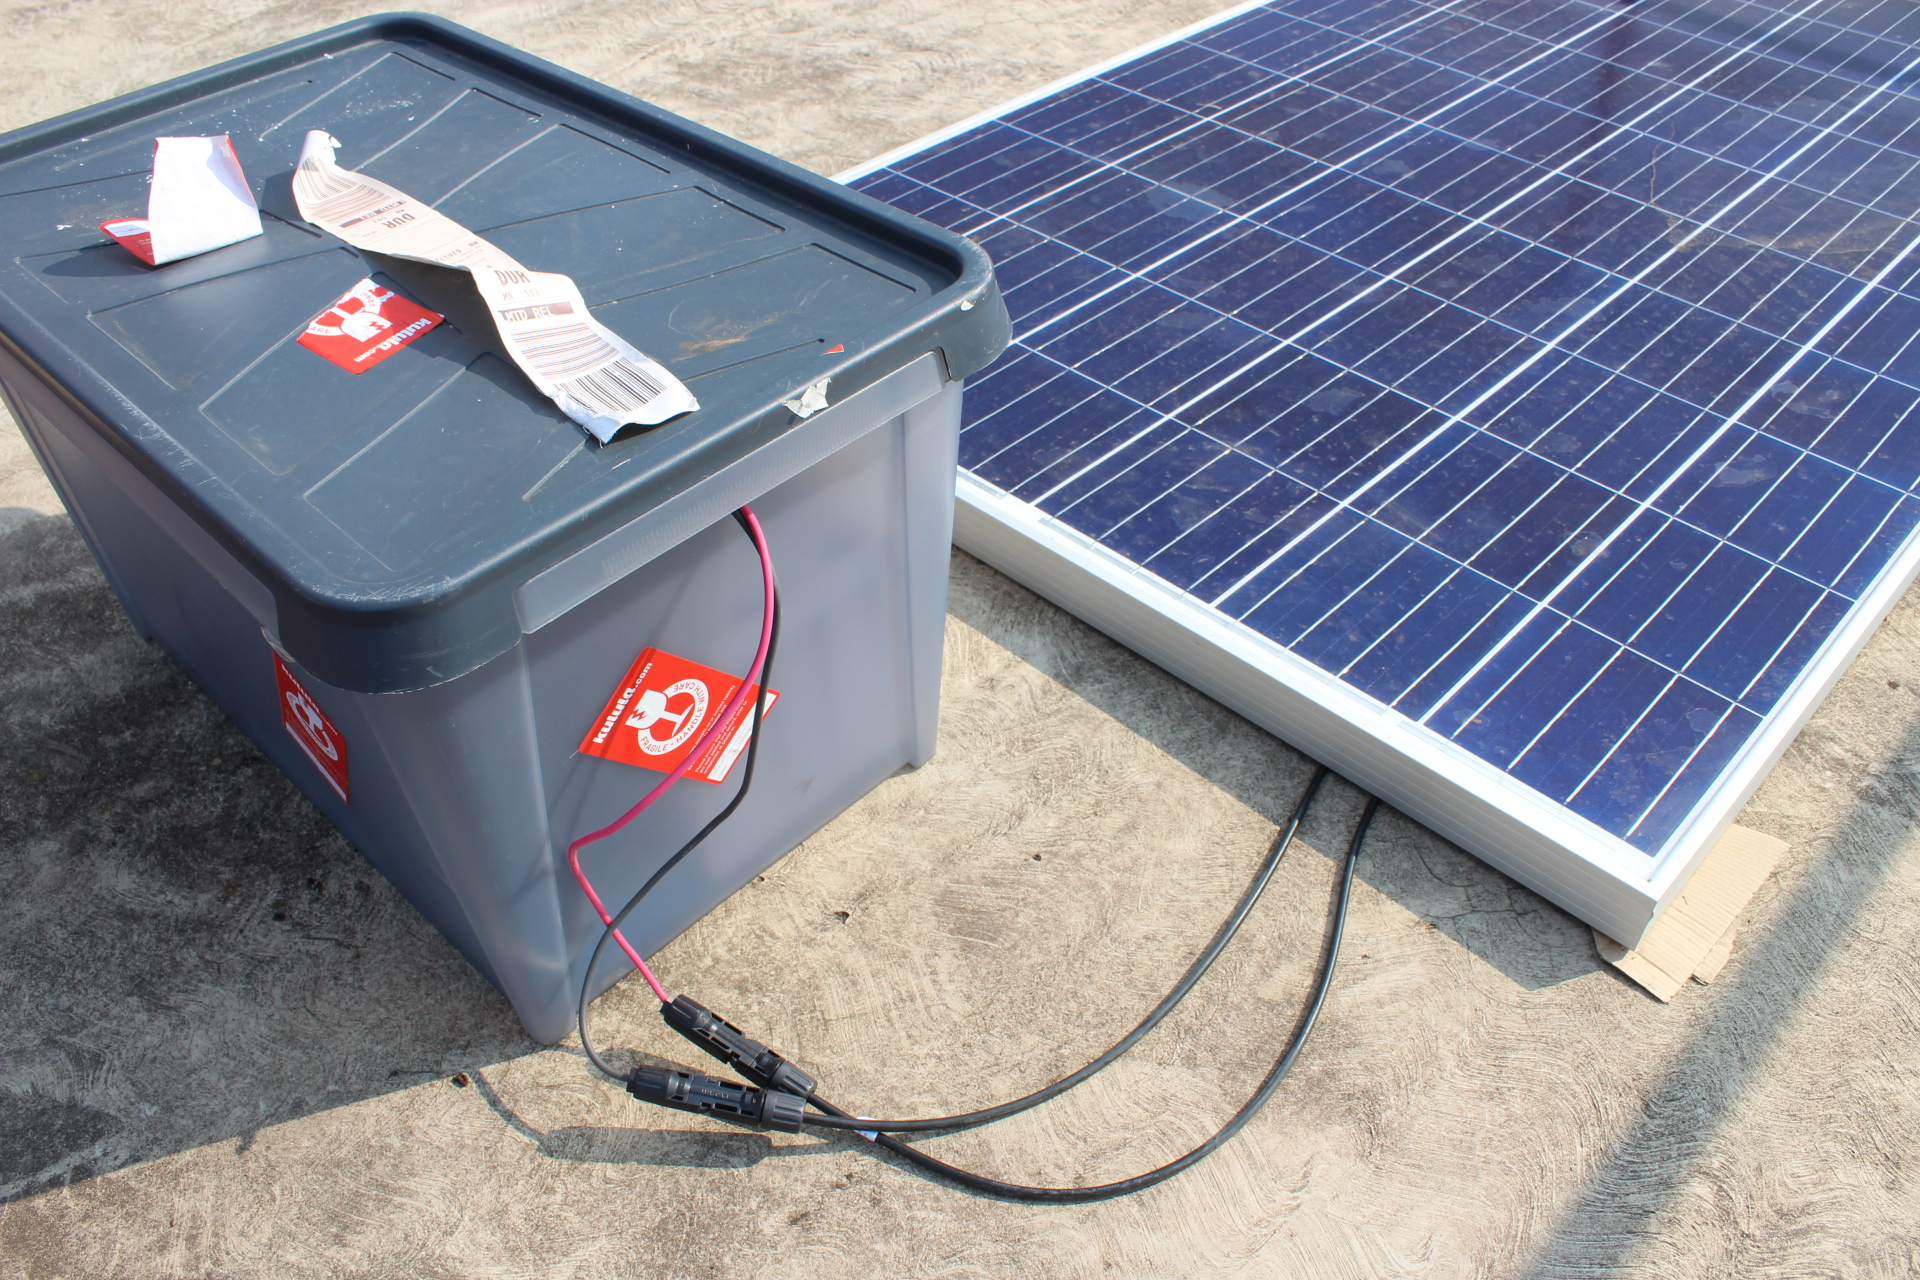
\includegraphics[width=0.8\linewidth]{Figures/rooftop1.JPG}
		\caption{Solar Panel and Weather Proof Electronics Enclosure}
		\label{Fig:Rooftop1}
	\end{center}
\end{figure}

\begin{figure}[h!]
	\begin{center}
		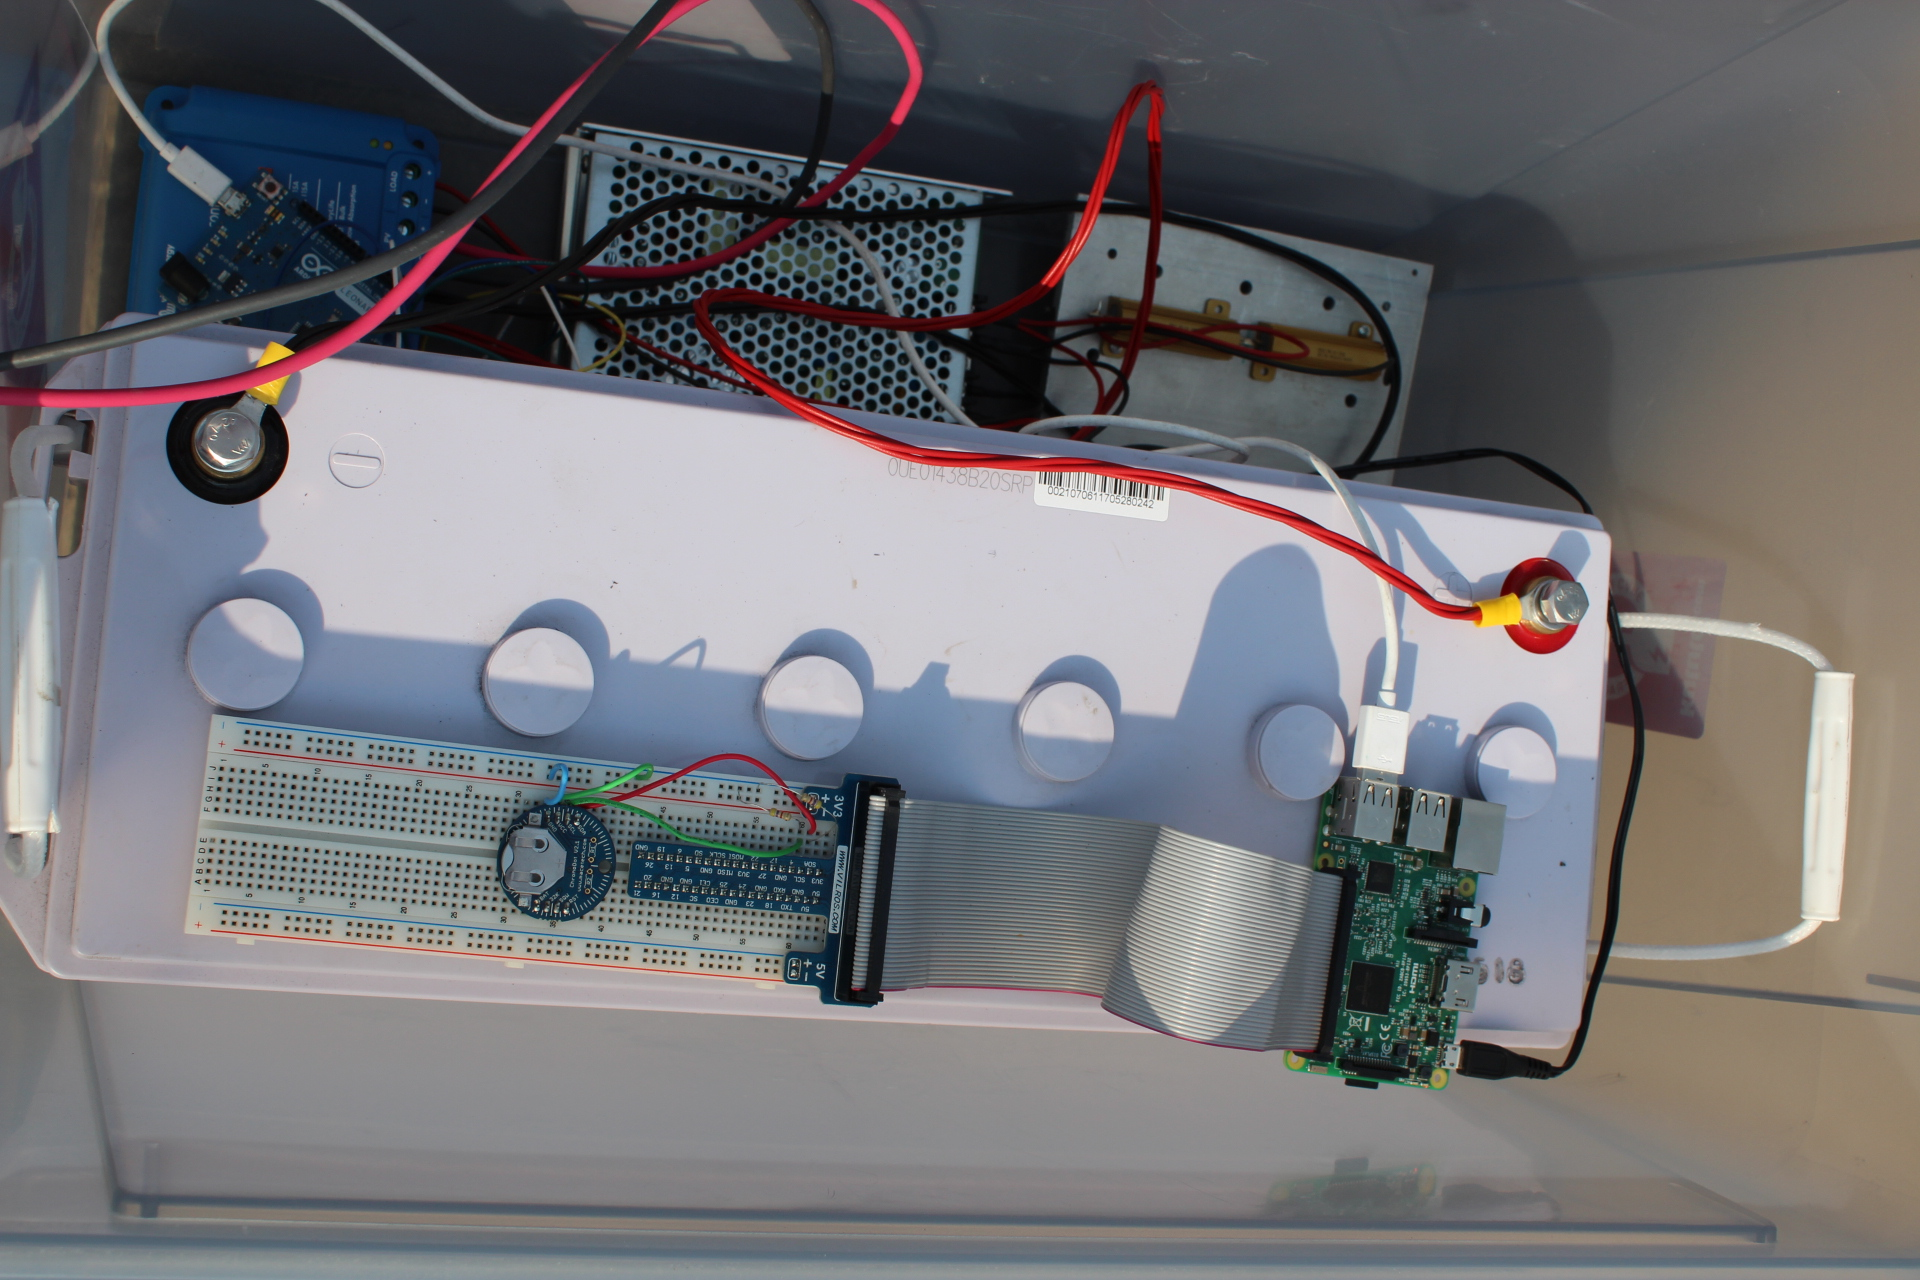
\includegraphics[width=1\linewidth]{Figures/rooftop2.JPG}
		\caption{Interior of the Weather Proof Enclosure}
		\label{Fig:Rooftop2}
	\end{center}
\end{figure}

\newpage
\subsection{Measurements and Results}

In order to interpret the data that was monitored from the system, a Python script was written to read the week's data files that were saved in the Rpi, extracted the parameters of interest and plotted them. The parameters of interest were:

\begin{enumerate}
	\item The battery voltage (V) in Volts,
	\item The battery current (I) in Amperes,
	\item The solar panel voltage (VPV) in Volts,
	\item The solar panel power (PPV) in Watts,
	\item The load current (IL) in Amperes, and
	\item The state of operation (CS).
\end{enumerate}

From the test set up in \autoref{Fig:Rooftop}, plots from \autoref{Fig:V} to \autoref{Fig:CS} are the results of parameters that were plotted respectively. All these measurements were taken during the time interval of the 18th to the 24th of September 2018. The system started running at approximately 12:00 pm on the 18th of September 2018 and it was operational up until it was switched off on the 24th of September 2018 round about 16:00 pm.\\
\autoref{Fig:V} illustrates the battery voltage vs. date measurement plot which shows the performance of the battery during that time interval of approximately a week.
\autoref{Fig:I} illustrates the battery current vs. date measurement plot.
\autoref{Fig:VPV} illustrates the solar panel voltage vs. date measurement plot.
\autoref{Fig:PPV} illustrates the solar panel power vs. date measurement plot.

All the plots from \autoref{Fig:V} to \autoref{Fig:PPV} are governed by the power law equation\footnote{http://www.sengpielaudio.com/calculator-ohm.htm} which is given by 

\begin{equation} \label{Power}
	\begin{split}
	P & = IV,
	\end{split}
\end{equation}
where P is the power in Watts (W), I is the current in Amperes (A) and V is the voltage in Volts (V). From these plots, during morning hours to the early afternoon hours, there is a pick up because of the high levels of radiation from the Sun. On the 22nd of September 2018, the weather in Durban was not as sunny as expected, thus, these parameters did not pick up to their maximum of the week and can also deduce from especially the battery voltage, battery current and solar panel power plots that during three of the days, the Sun's radiation was at minimum. \\

The maximum of each parameter that was measured during this interval was $\approx$14 V, $\approx$12.5 A, $\approx$40 V and $\approx$230 W respectively. The minimum values which were measured for each each parameter during this interval was $\approx$12 V, $\approx$-2.5 A, $\approx$0.08 V and $\approx$0 W respectively. Assuming that the second battery was also functional in the system, the performance of the system was going to increase by at least \SI{40}{\percent}. 

\begin{figure}[h!]
	\begin{center}
		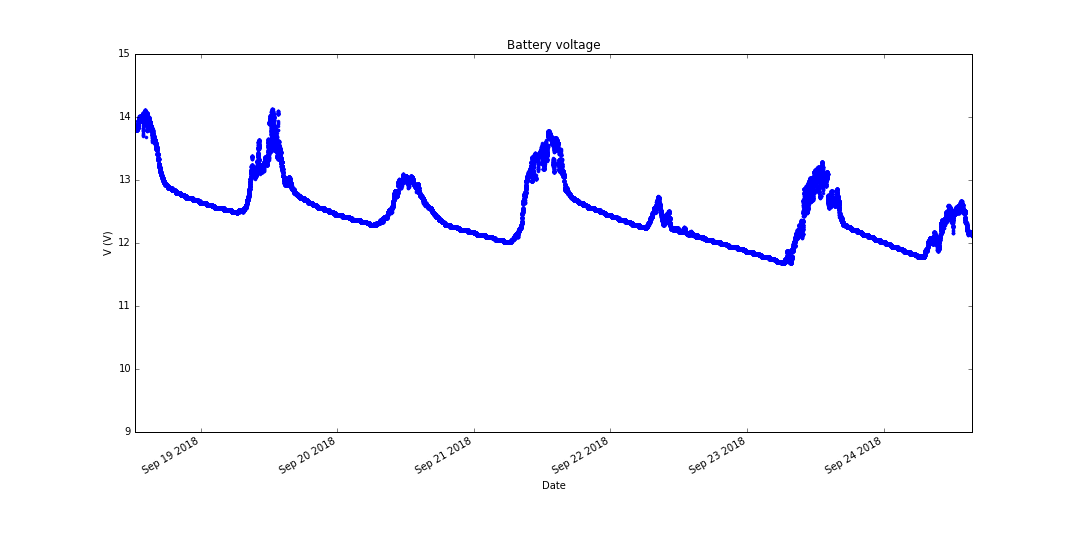
\includegraphics[width=1\linewidth]{Figures/V.png}
		\caption{Voltage Plot of the Whole Week}
		\label{Fig:V}
	\end{center}
\end{figure}

\begin{figure}[h!]
	\begin{center}
		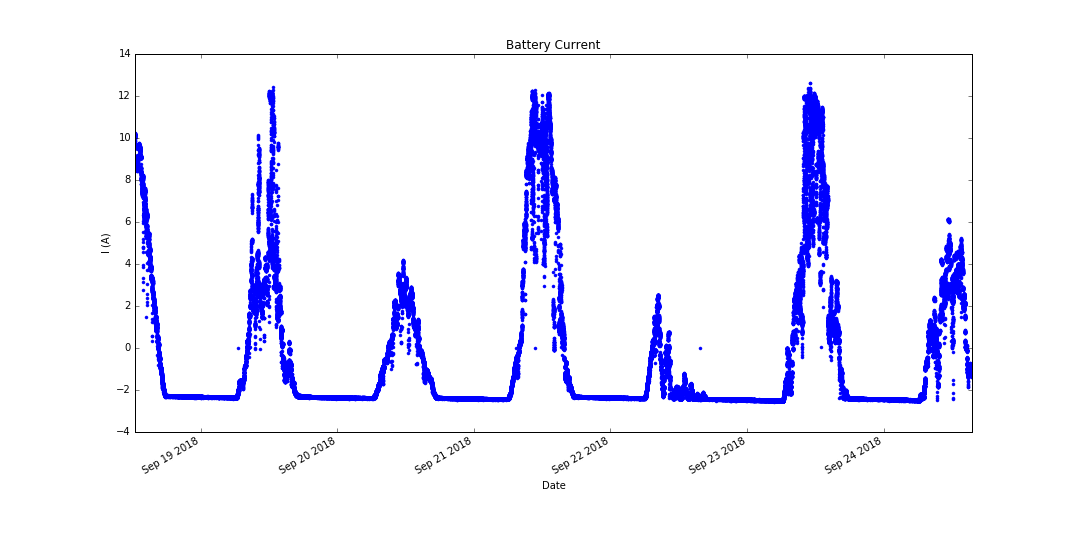
\includegraphics[width=1\linewidth]{Figures/I.png}
		\caption{Current Plot of the Whole Week}
		\label{Fig:I}
	\end{center}
\end{figure}

\begin{figure}[h!]
	\begin{center}
		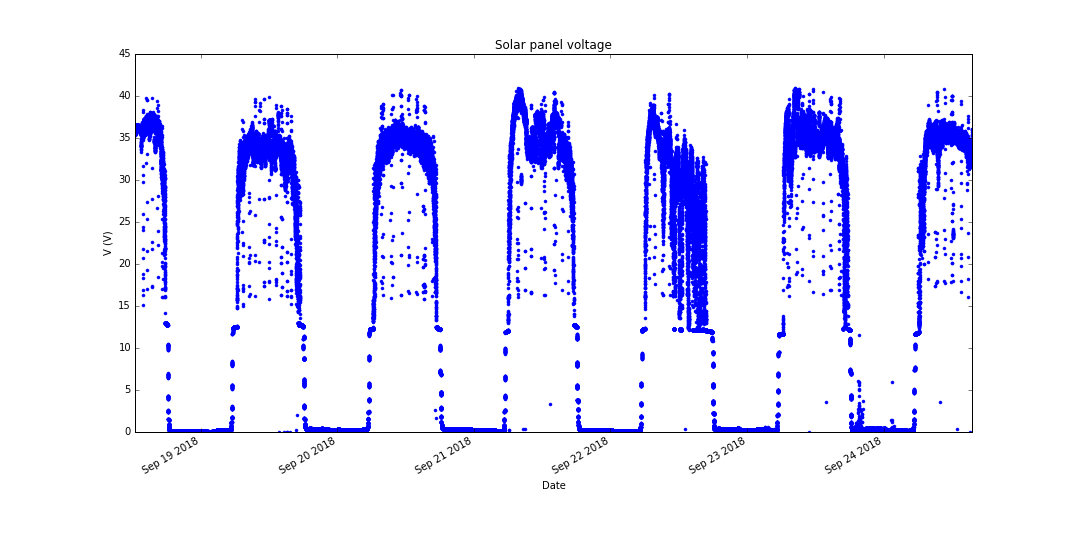
\includegraphics[width=1\linewidth]{Figures/VPV.png}
		\caption{Panel Voltage Plot of the Whole Week}
		\label{Fig:VPV}
	\end{center}
\end{figure}

\begin{figure}[h!]
	\begin{center}
		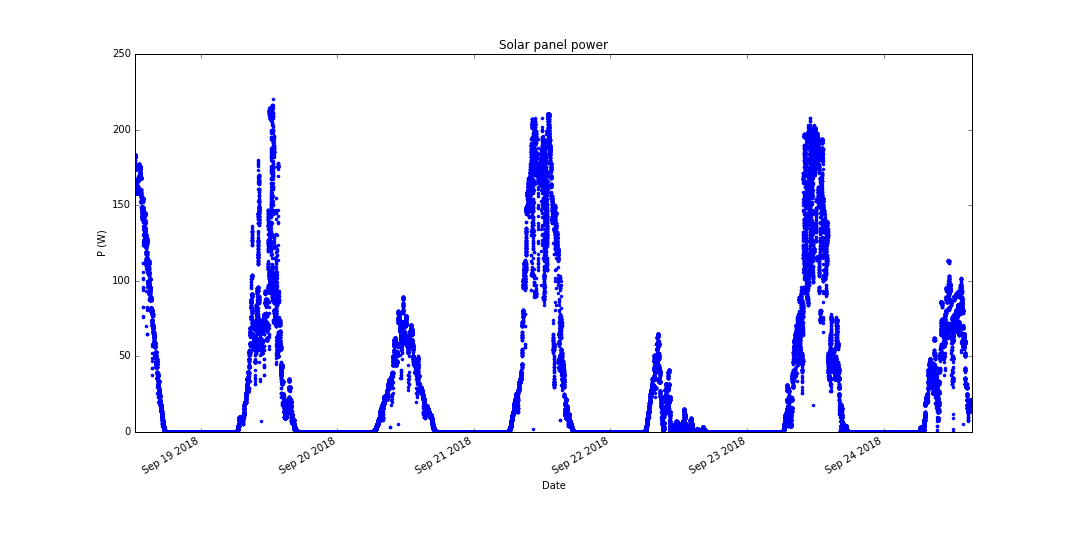
\includegraphics[width=1\linewidth]{Figures/PPV.png}
		\caption{Panel Power Plot of the Whole Week}
		\label{Fig:PPV}
	\end{center}
\end{figure}


\autoref{Fig:IL} illustrates the load current vs. date measurement plot. The load current remained the same for most of the days. It peaked on the 19th, 21st and 23rd of September 2018 as illustrated by the plot. It was expected that the load draws 2 A at +12 VDC, but because the load power from the solar regulator went via a DC-DC converter to the actual load of \SI{6}{\ohm}, the DC-DC converter also dissipated an amount of power which also had an effect in the increasing value of the load current. The Sun's radiation was also a contributing factor. The load current flactuated between a minimum of 2 A and a maximum of 3 A.

\begin{figure}[h!]
	\begin{center}
		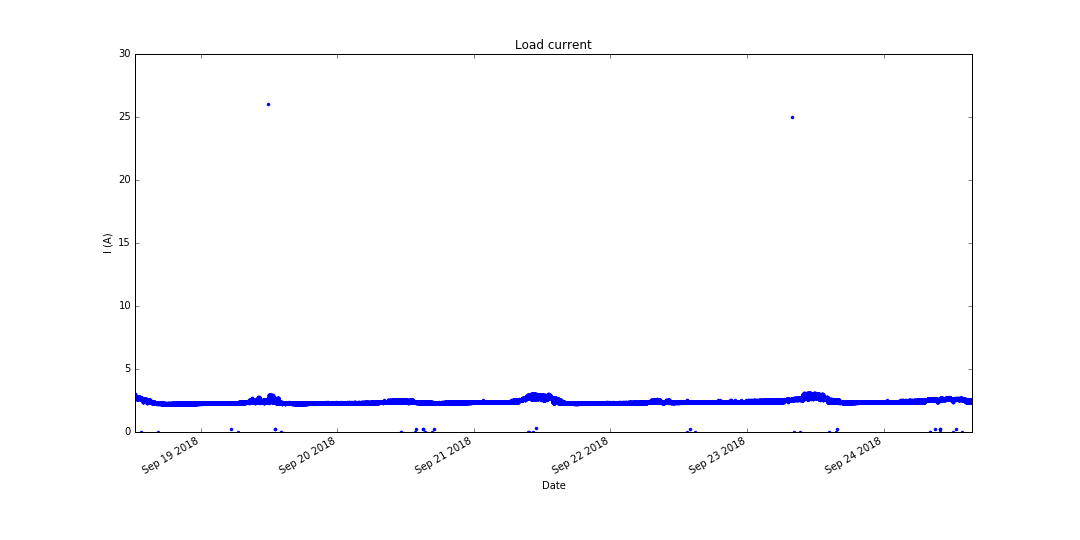
\includegraphics[width=1\linewidth]{Figures/IL.png}
		\caption{Load Current Plot of the Whole Week}
		\label{Fig:IL}
	\end{center}
\end{figure}

\autoref{Fig:CS} illustrates the measurement plot of the state of operation vs. date. \autoref{table:CS}\footnote{http://www.tiarora.no/Victron/VE.Direct-Protocol-3.24.pdf} shows the state of operation of the system and measurement possible values. Looking closely into the operation state plot, there is a dot at the value 4 on the 19th of September 2018 which is what would be expected if the system was at its very best performance, instead it is at the value of 3 most when the Sun's radiation is high and at 0 when there is no radiation from the Sun. It can also be seen on the 21st of September 2018, the battery value went to 1, which implies low power.

\begin{figure}[h!]
	\begin{center}
		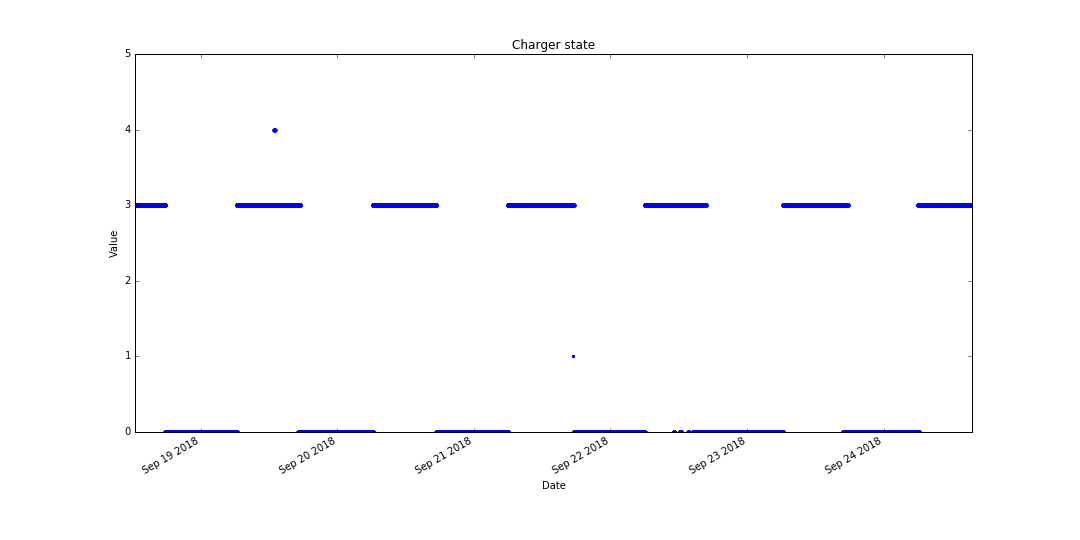
\includegraphics[width=1\linewidth]{Figures/CS.png}
		\caption{Charger State of Operation Plot of the Whole Week}
		\label{Fig:CS}
	\end{center}
\end{figure}

\begin{table}[h!]
	\centering
	\begin{tabular}{|c | c | c | c|} 
		\hline
		State & Value \\ [0.5ex] 
		\hline
		Off & 0  \\
		\hline
		Low Power & 1 \\
		\hline
		Fault & 2 \\
		\hline
		Bulk & 3 \\
		\hline
		Absorption & 4 \\ [1ex] 
		\hline
		Float & 5 \\ [1ex] 
		\hline
	\end{tabular}
	\caption{State of Operation and Possible Values}
	\label{table:CS}
\end{table}

\newpage
The battery reached the natural absorption rate only once as shown in \autoref{Fig:CS} by the value of 4 on the 19th of September. This means that the 300 W solar panel that was available was not sufficient enough to even fully charge one battery. If the battery was being fully charged, a value of 4 would be expected in most of the days compared to having a value of 3 almost every day, and the system would not shut down during night hours if the battery reached the natural absorption rate.

The discussed results have paved a way to future tests, designs and implementation, since the solar panel monitoring system is aimed at being integrated with the ALBATROS data acquisition (DAQ) system.

\newpage
\section{Solar Regulator Radio Frequency Interference (RFI)}
\subsection{Discussion}
The solar regulator uses the switch mode to charge the battery. This switching mode of charging the battery creates RFI which is a threat to radio frequency systems. So, RFI measurements had to be done in order to know how much RFI the solar regulator generates, at what frequency and find ways to reject all the RFI that is radiated. The measurements were done in the lab using the same battery that was used to do the previous test, the same solar regulator. The DC-DC converter was removed and a \SI{6}{\ohm} load was connected on its own to the solar regulator. Instead of using the solar panel, the bench power supply unit (PSU) was used to provide power to the solar regulator. A biconical antenna\footnote{https://www.aaronia.com/products/antennas/BicoLOG-20300/} was an input to the spectrum analyser in order to analyse the RFI which was generated.  The spectrum analyser saves the datafile as .csv files. A python script had to be written to convert and plot the measurements accordingly. The test setup of the solar regulator RFI measurement is illustrated by the block diagram of the test setup in \autoref{Fig:BlockDiagram} and the test setup is shown in \autoref{Fig:setup}.\\

\begin{figure}[h!]
	\begin{center}
		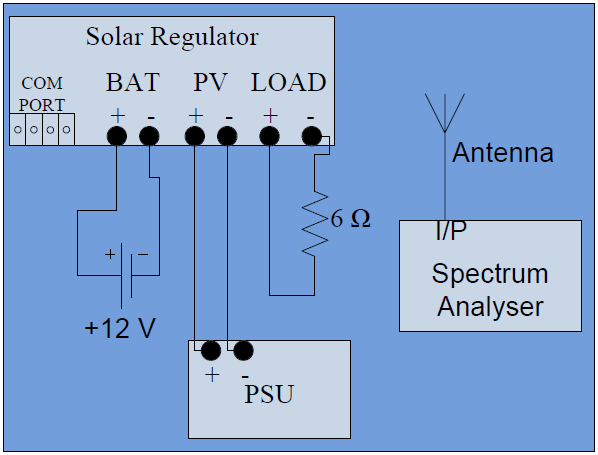
\includegraphics[width=0.7\linewidth]{Figures/RFI.PNG}
		\caption{RFI Test Set Up Block Diagram}
		\label{Fig:BlockDiagram}
	\end{center}
\end{figure}

\begin{figure}[h!]
	\begin{center}
		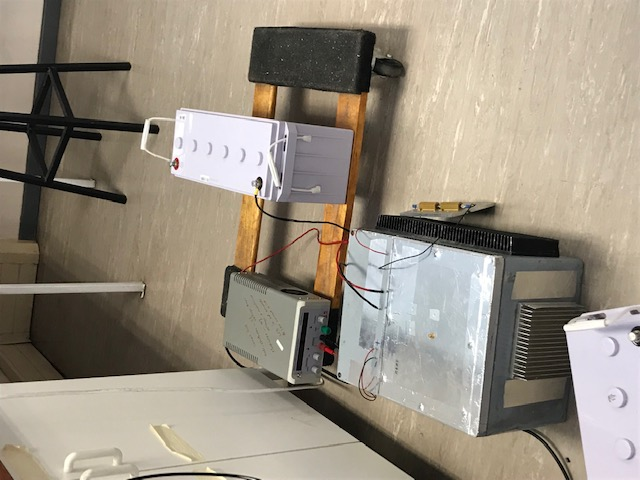
\includegraphics[width=0.6\linewidth, angle=-90]{Figures/IMG_3784.jpg}
		\caption{RFI Test Set Up}
		\label{Fig:setup}
	\end{center}
\end{figure}

\newpage
\subsection{Measurements and Results}
When doing this measurement a thick aluminium RFI tight box was used in order to measure RFI and to solve the problem. The RF feed throughs were drilled for and used to make connections from the components inside to the components outside the box. An SubMiniature version A (SMA) female to female connector was drilled for and was used for the antenna-spectrum analyser connection. The test was done with the antenna enclosed inside the box together with the solar regulator and load. and secondly the test was done with the antenna outside the box with the solar regulator left inside the box. This measurement was done at different frequencies and with the solar regulator connected and disconnected, this was done to validate the results. 

\subsection{Antenna Inside the Box}
This was done to measure the RFI that was generated by the solar regulator with the antenna inside the box. All the RFI measurement plots are power level (dBm) vs. frequency (MHz) plots. \autoref{Fig:1} shows the solar regulator RFI plot at 125 MHz. \autoref{Fig:125} shows the RFI measurement plot at 125 MHz with the charger switched on and off and \autoref{Fig:dif125} is the difference between the two solar regulator states plot. \autoref{Fig:1} shows that the solar regulator switches at a frequency range of $\approx$ 30 MHz to $\approx$ 40 MHz which generates the RFI. \\

From \autoref{Fig:2} the same information is deduced about the solar regulator RFI and at the range of $\approx$150 MHz and $\approx$170 MHz, that is suggested to be the two way land mobile\footnote{http://www.gb.nrao.edu/IPG/Interference/125-200MHz.pdf}. \autoref{Fig:450on} illustrates the plot of RFI generated when the solar regulator is switched on and \autoref{Fig:450off} illustrates the plot of the RFI generated when the solar regulator is swiched off. What the antenna measured at $\approx$400 MHz to $\approx$430 MHz is suggested to be the the frequency range of mobile phones services including mobile data services\footnote{http://www.internet.org.za/SABRE-1.pdf}. Additionally, this frequency range of solar regulator switching falls under the ALBATROS operating frequency ranges which will degrade the RF signal detected. Thus, it is crucial to overcome this RFI.

\begin{figure}[!htb]
	\centering
	\begin{subfigure}{.5\textwidth}
		\centering
		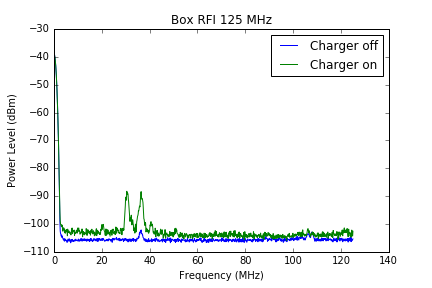
\includegraphics[width=.9\linewidth]{Figures/box_rfi_charger_on_125mhz_1.png}
		\caption{A Plot of Two States (On/Off) of a Solar Regulator at 125 MHz}
		\label{Fig:125}
	\end{subfigure}%
	\begin{subfigure}{.5\textwidth}
		\centering
		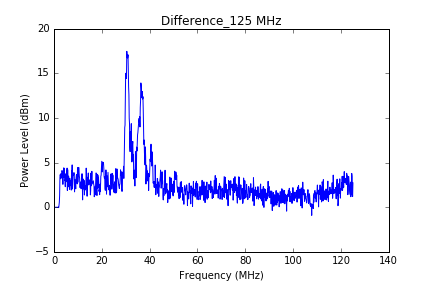
\includegraphics[width=.9\linewidth]{Figures/1Difference_125mhz.png}
		\caption{A Plot of the Difference Between the Two Solar Regulator States}
		\label{Fig:dif125}
	\end{subfigure}
	\caption{A Plot of Solar Regulator RFI at 125 MHz with the Antenna Inside the Box}
	\label{Fig:1}
\end{figure}

\begin{figure}[!htb]
	\centering
	\begin{subfigure}{.5\textwidth}
		\centering
		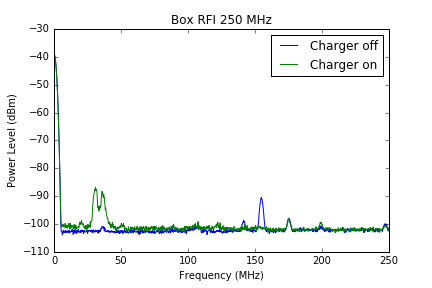
\includegraphics[width=.9\linewidth]{Figures/box_rfi_charger_on_250mhz_1.png}
		\caption{A Plot of Two States (On/Off) of a Solar Regulator at 250 MHz}
		\label{Fig:250}
	\end{subfigure}%
	\begin{subfigure}{.5\textwidth}
		\centering
		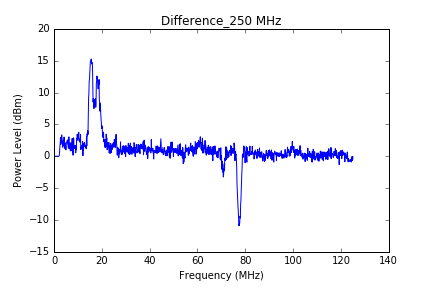
\includegraphics[width=.9\linewidth]{Figures/1Difference_250mhz.png}
		\caption{A Plot of the Difference Between the Two Solar Regulator States}
		\label{Fig:dif250}
	\end{subfigure}
	\caption{A Plot of Solar Regulator RFI at 250 MHz with the Antenna Inside the Box}
	\label{Fig:2}
\end{figure}


\begin{figure}[!htb]
	\centering
	\begin{subfigure}{.5\textwidth}
		\centering
		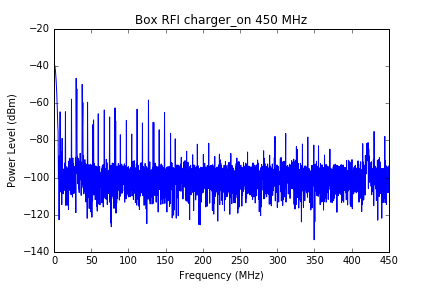
\includegraphics[width=.9\linewidth]{Figures/box_rfi_charger_on_450mhz.png}
		\caption{A Plot of the Solar Regulator RFI at 450 MHz with the Sola Regulator Switched On}
		\label{Fig:450on}
	\end{subfigure}%
	\begin{subfigure}{.5\textwidth}
		\centering
		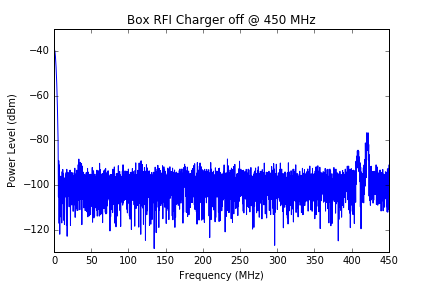
\includegraphics[width=.9\linewidth]{Figures/box_rfi_charger_off_450mhz.png}
		\caption{A Plot of the Solar Regulator RFI at 450 MHz with the Sola Regulator Switched Off}
		\label{Fig:450off}
	\end{subfigure}
	\caption{A Plot of RFI of Two States of the Solar Regulator at 450 MHz with the Antenna Inside the Box}
	\label{Fig:3}
\end{figure}

\newpage
\subsection{Antenna Outside the Box}

This measurement was done in the lab to measure the RFI that was generated by the solar regulator with the antenna outside the box. The aim of placing the antenna outside the box is to check whether the antenna will detect the switching of the solar regulator or not since the solars regulator was inside the box. \\

\autoref{Fig:1251} shows the RFI which was measured in the lab environment. It is clear from the frequency range from $\approx$80 MHz to $\approx$110 MHz that the frequency modulation (FM) band was detected. From \autoref{Fig:dif1251}, at the frequency range of $\approx$ 30 MHz to $\approx$ 40 MHz, we no longer detect the solar regulator RFI, which means that the aluminium box that enclosed the solar regulator is RFI tight i.e. RFI which is generated in the box can not affect any systems outside of the box. As well as on \autoref{Fig:5}, the solar regulator is not detected, only the RFI generated by the environment is detected. This means that the solar regulator RFI problem was solved by using an RFI tight aluminium box.

\begin{figure}[!htb]
	\centering
	\begin{subfigure}{.5\textwidth}
		\centering
		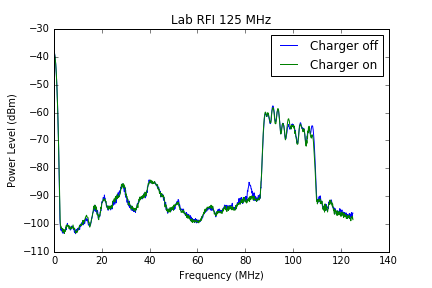
\includegraphics[width=.9\linewidth]{Figures/lab_rfi_charger_on_off_125MHz.png}
		\caption{RFI of the Environment at 125 MHz}
		\label{Fig:1251}
	\end{subfigure}%
	\begin{subfigure}{.5\textwidth}
		\centering
		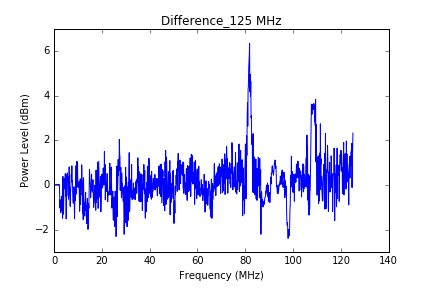
\includegraphics[width=.9\linewidth]{Figures/Difference_125mhz.png}
		\caption{A Plot of the Difference Between the Two Solar Regulator States}
		\label{Fig:dif1251}
	\end{subfigure}
	\caption{Enviroment RFI at 125 MHz}
	\label{Fig:4}
\end{figure}

\begin{figure}[!htb]
	\centering
	\begin{subfigure}{.5\textwidth}
		\centering
		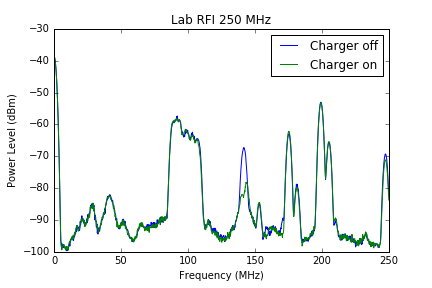
\includegraphics[width=.9\linewidth]{Figures/lab_rfi_charger_on_off_250MHz.png}
		\caption{RFI of the Environment at 250 MHz}
		\label{Fig:2501}
	\end{subfigure}%
	\begin{subfigure}{.5\textwidth}
		\centering
		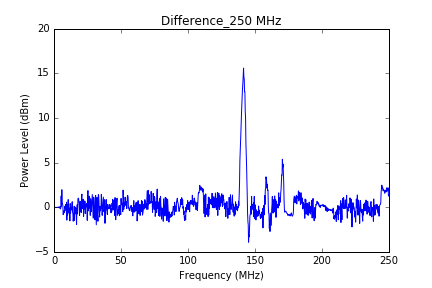
\includegraphics[width=.9\linewidth]{Figures/Difference_250mhz.png}
		\caption{A Plot of the Difference Between the Two Solar Regulator States}
		\label{Fig:dif2501}
	\end{subfigure}
	\caption{Enviroment RFI at 250 MHz}
	\label{Fig:5}
\end{figure}

When the antenna is outside of the box, it is susceptible to all unknown RFI sources in the environment. The visible differences between the charger on/off states are not necessarily due to the solar regulator, they could very well come from time-varying environmental RFI as well. The differences in these measurements give an upper limit or
worst case scenario on charger RFI leaking out of the box, but these measurements can not really be trusted  quantitatively.
	
\newpage	
\section{System Levels}

From \autoref{Fig:levels}, the noise factor was calculated for a single polarisation. The overall system has six stages, The FEE, the coaxial cable, the bias tee, the HPF, the LPF and an amplifier. 
\begin{figure}[h!]
	\begin{center}
 		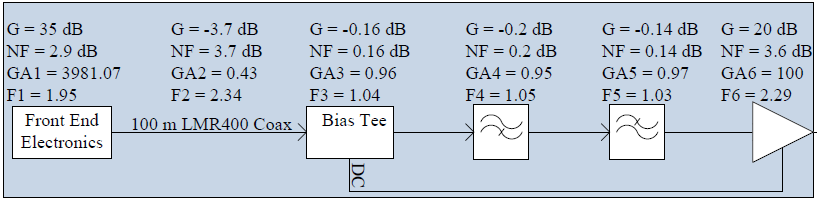
\includegraphics[width=1\linewidth]{Figures/levels.PNG}
		\caption{Overall System Levels for the Receiver}
		\label{Fig:levels}
	\end{center}
\end{figure}

The values of gain and noise figure were deduced from the components datasheets. The overall system noise factor was determined by the Friiss' Formula which is given by
\begin{equation} \label{eq2.2}
	\begin{split}
	F & = F_{1} + \frac{F_{2} - 1}{G_{A1}} + \frac{F_{3} - 1}{G_{A1} G_{A2}} + \frac{F_{4} - 1}{G_{A1} G_{A2} G_{A3}} +... + \frac{F_{n} - 1}{G_{A1} G_{A2} \times ... \times G_{n-1}}, \\[0.1cm]				
	\end{split}
\end{equation}
where F is the noise factor, G\textsubscript{Ax} (x = 1, 2, 3, ...) is the gain of each stage. The noise factor was calculated to be 1.951. F can be expressed in dB using 
		
\begin{equation} \label{eq2.3}
	\begin{split}
	NF & = 10 \log F,				
	\end{split}
\end{equation}
where NF is the noise figure in dB. NF was calculated to be 2.9 dB. The obtained F can also be used to calculate the equivalent noise temperature of the system (T\textsubscript{e}) which is given by 

\begin{equation} \label{eq2.9}
\begin{split}
T_{e} & = (F-1)T_{0},				
\end{split}
\end{equation}
where (T\textsubscript{0}) is a standard temperature of \SI{290}{\kelvin}. T\textsubscript{e} was calculated to be \SI{275.79}{\kelvin}. The overall gain (G\textsubscript{T}) of the system was then calculated using 
	
\begin{equation} \label{eq2.4}
	\begin{split}
	G_{T} & = G_{1} + G_{2} + G_{3} + ... + G_{n}, 				
	\end{split}
\end{equation}
which resulted in the overall system gain of 51.8 dB.

\chapter{Conclusion and Recommendations}

\autoref{Fig:auto} and \autoref{Fig:fringes} shows the initial results from the two interferometric array currently installed in Marion Island. 

These results are an encouraging factor to proceed with the development of the autonomous stations.\autoref{Fig:auto} shows the raw ALBATROS-EGG autospectra which where the waterfall plot was taken from one polarization (pol0) over an interval of 3 days. The Galaxy rising/setting is clearly visible in the structure. There are also ripples in frequency because of uncalibrated data, and the ripples arise from reflections in the cables. There is a qualitative difference between daytime and nighttime data and this shows that the contamination from shortwave radio drops off significantly at night, when the ionosphere becomes quieter.

\begin{figure}[h!]
	\begin{center}
		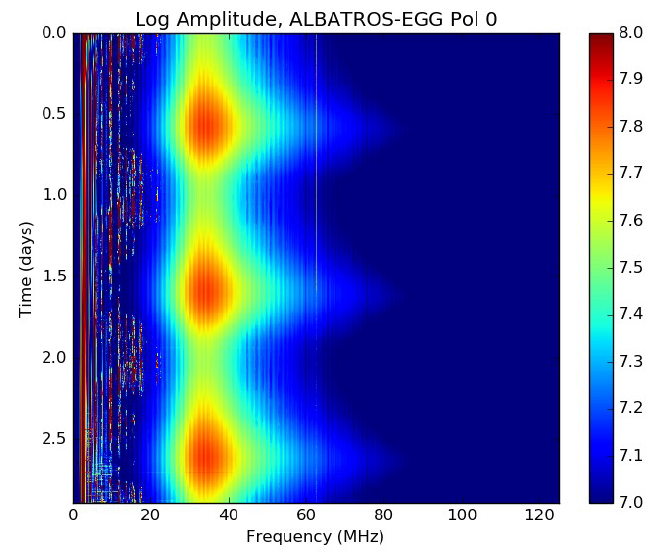
\includegraphics[width=0.8\linewidth]{Figures/Raw-ALBATROS-autospectra.PNG}
		\caption{Raw ALBATROS-EGG Autospectra}
		\label{Fig:auto}
	\end{center}
\end{figure}

\autoref{Fig:fringes} shows the first fringes that were detected by the the ALBATROS-EGG. It is dinstictly visible from \autoref{Fig:fringes} that fringes show recurrent structure down to a frequency of as low as 10 MHz without data processing or data cuts.

\begin{figure}[ht!]
	\begin{center}
		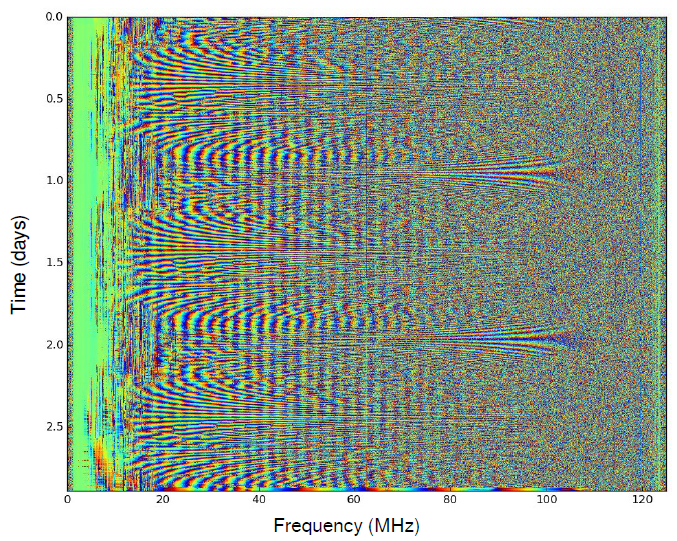
\includegraphics[width=1\linewidth]{Figures/First-fringes-of-ALBATROS-EGG.PNG}
		\caption{First Fringes from ALBATROS-EGG}
		\label{Fig:fringes}
	\end{center}
\end{figure}



It has been discovered that the receiver system needs more power in order to function without running short of power. The following needs to be considered and done for the deployment in 2019,

\begin{enumerate}
	\item An array of solar panels is needed since the weather in Marion Island is more cloudy than sunny.
	
	\begin{enumerate}
		\item The first thing that needs to be done is to test the solar power system for at least a week again, now with two batteries connected in order to observe the improvement, then plot the results and compare them with the results which were measured in September 2018.
		
		\item From the resuts that will be measured during that period, it can be deduced how much of solar panel array power would be needed in order for our system to survive the Marion Island weather since the ALBATROS-EGG is powered using two batteries.
	\end{enumerate}
	
\item The Mini Circuits amplifier (ZX60-V63) which is connected at the backend of the system has an operating frequency of 0.05 - 6 GHz which is too wide for the ALBATROS-EGG system which operates between 1.2 - 81 MHz. A suggested amplifier to replace the ZX60-V63 (with NF = 3.6 dB and G = 20 dB) is the Mini Circuits ZFL-500LN+\footnote{https://www.minicircuits.com/pdfs/ZFL-500LN+.pdf} which operates between 0.1 - 500 MHz (NF = 2.9 and G = 24 dB). 

\begin{figure}[ht!]
	\begin{center}
		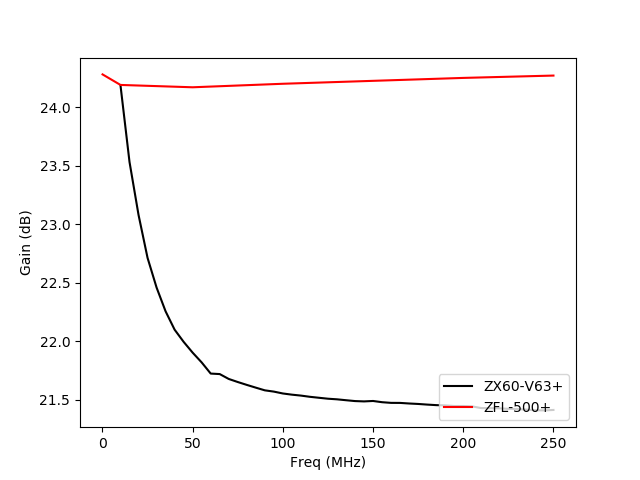
\includegraphics[width=0.8\linewidth]{Figures/foo.png}
		\caption{The comparison plot of S21 (gain) for the currently used amplifier and the proposed replacement amplifier.}
		\label{Fig:foo}
	\end{center}
\end{figure}

\item The integrated system of the receiver must be tested in the reverb chambers before the deployment to ensure functionality of the proposed changes.

\item Determining the lowest frequency at which we can recover sky signal. 

\item Understanding the signal rolloff below ~20 MHz. It is not yet of certainty if the antenna response is lost, or if there's a roll-off associated with the FEE modules or any other modules associated with the system.

\end{enumerate}.\\
Measurements of the proposed power system were discussed and how these can be improved for future deployment. The consistency of results proved that there is still more room for improvement. The major problem of the power system was which is solar regulator RFI was observed and the feasible solution was presented. It has been discussed that the development of the power system for the autonomous stations will be furtherly investigated since the project is ongoing.

\newpage		
\bibliography{References}		
%\bibliographystyle{agsm}
\bibliographystyle{unsrt}
\addcontentsline{toc}{section}{\numberline{}References}


\end{document}